
\chapter{基于双时相遥感影像风格解缠和内容细化增强遥感变化检测方法}
\section{引言}
近年来,基于深度学习的算法在遥感图像变化检测中取得了显著进展,特别是卷积神经网络(CNN)~\cite{Chen2020DASNetDA,Fang2021SNUNetCDAD}和Transformer架构~\cite{chen_remote_2022,zhang_swinsunet_2022}的应用。然而,变化检测任务中的一个关键挑战依然存在:双时相图像由于光照、季节或传感器噪声的变化,常常包含显著的风格差异。这些因素引入了不相关的特征级扰动,从而降低了检测精度。本章通过UMAP算法~\cite{McInnes2018UMAPUM}对五个数据集进行分析,并在图~\ref{fig:domain_vis}中可视化,证实了这一点。观察到双时相特征金字塔中的低级特征存在明显的域间隙。由于模型难以处理大的域间隙,这种与风格相关的干扰严重影响了变化检测任务。因此,有效解耦和利用内容与风格特征,成为提高精度和鲁棒性的关键挑战。


\begin{figure}[!htbp]
	\centering
	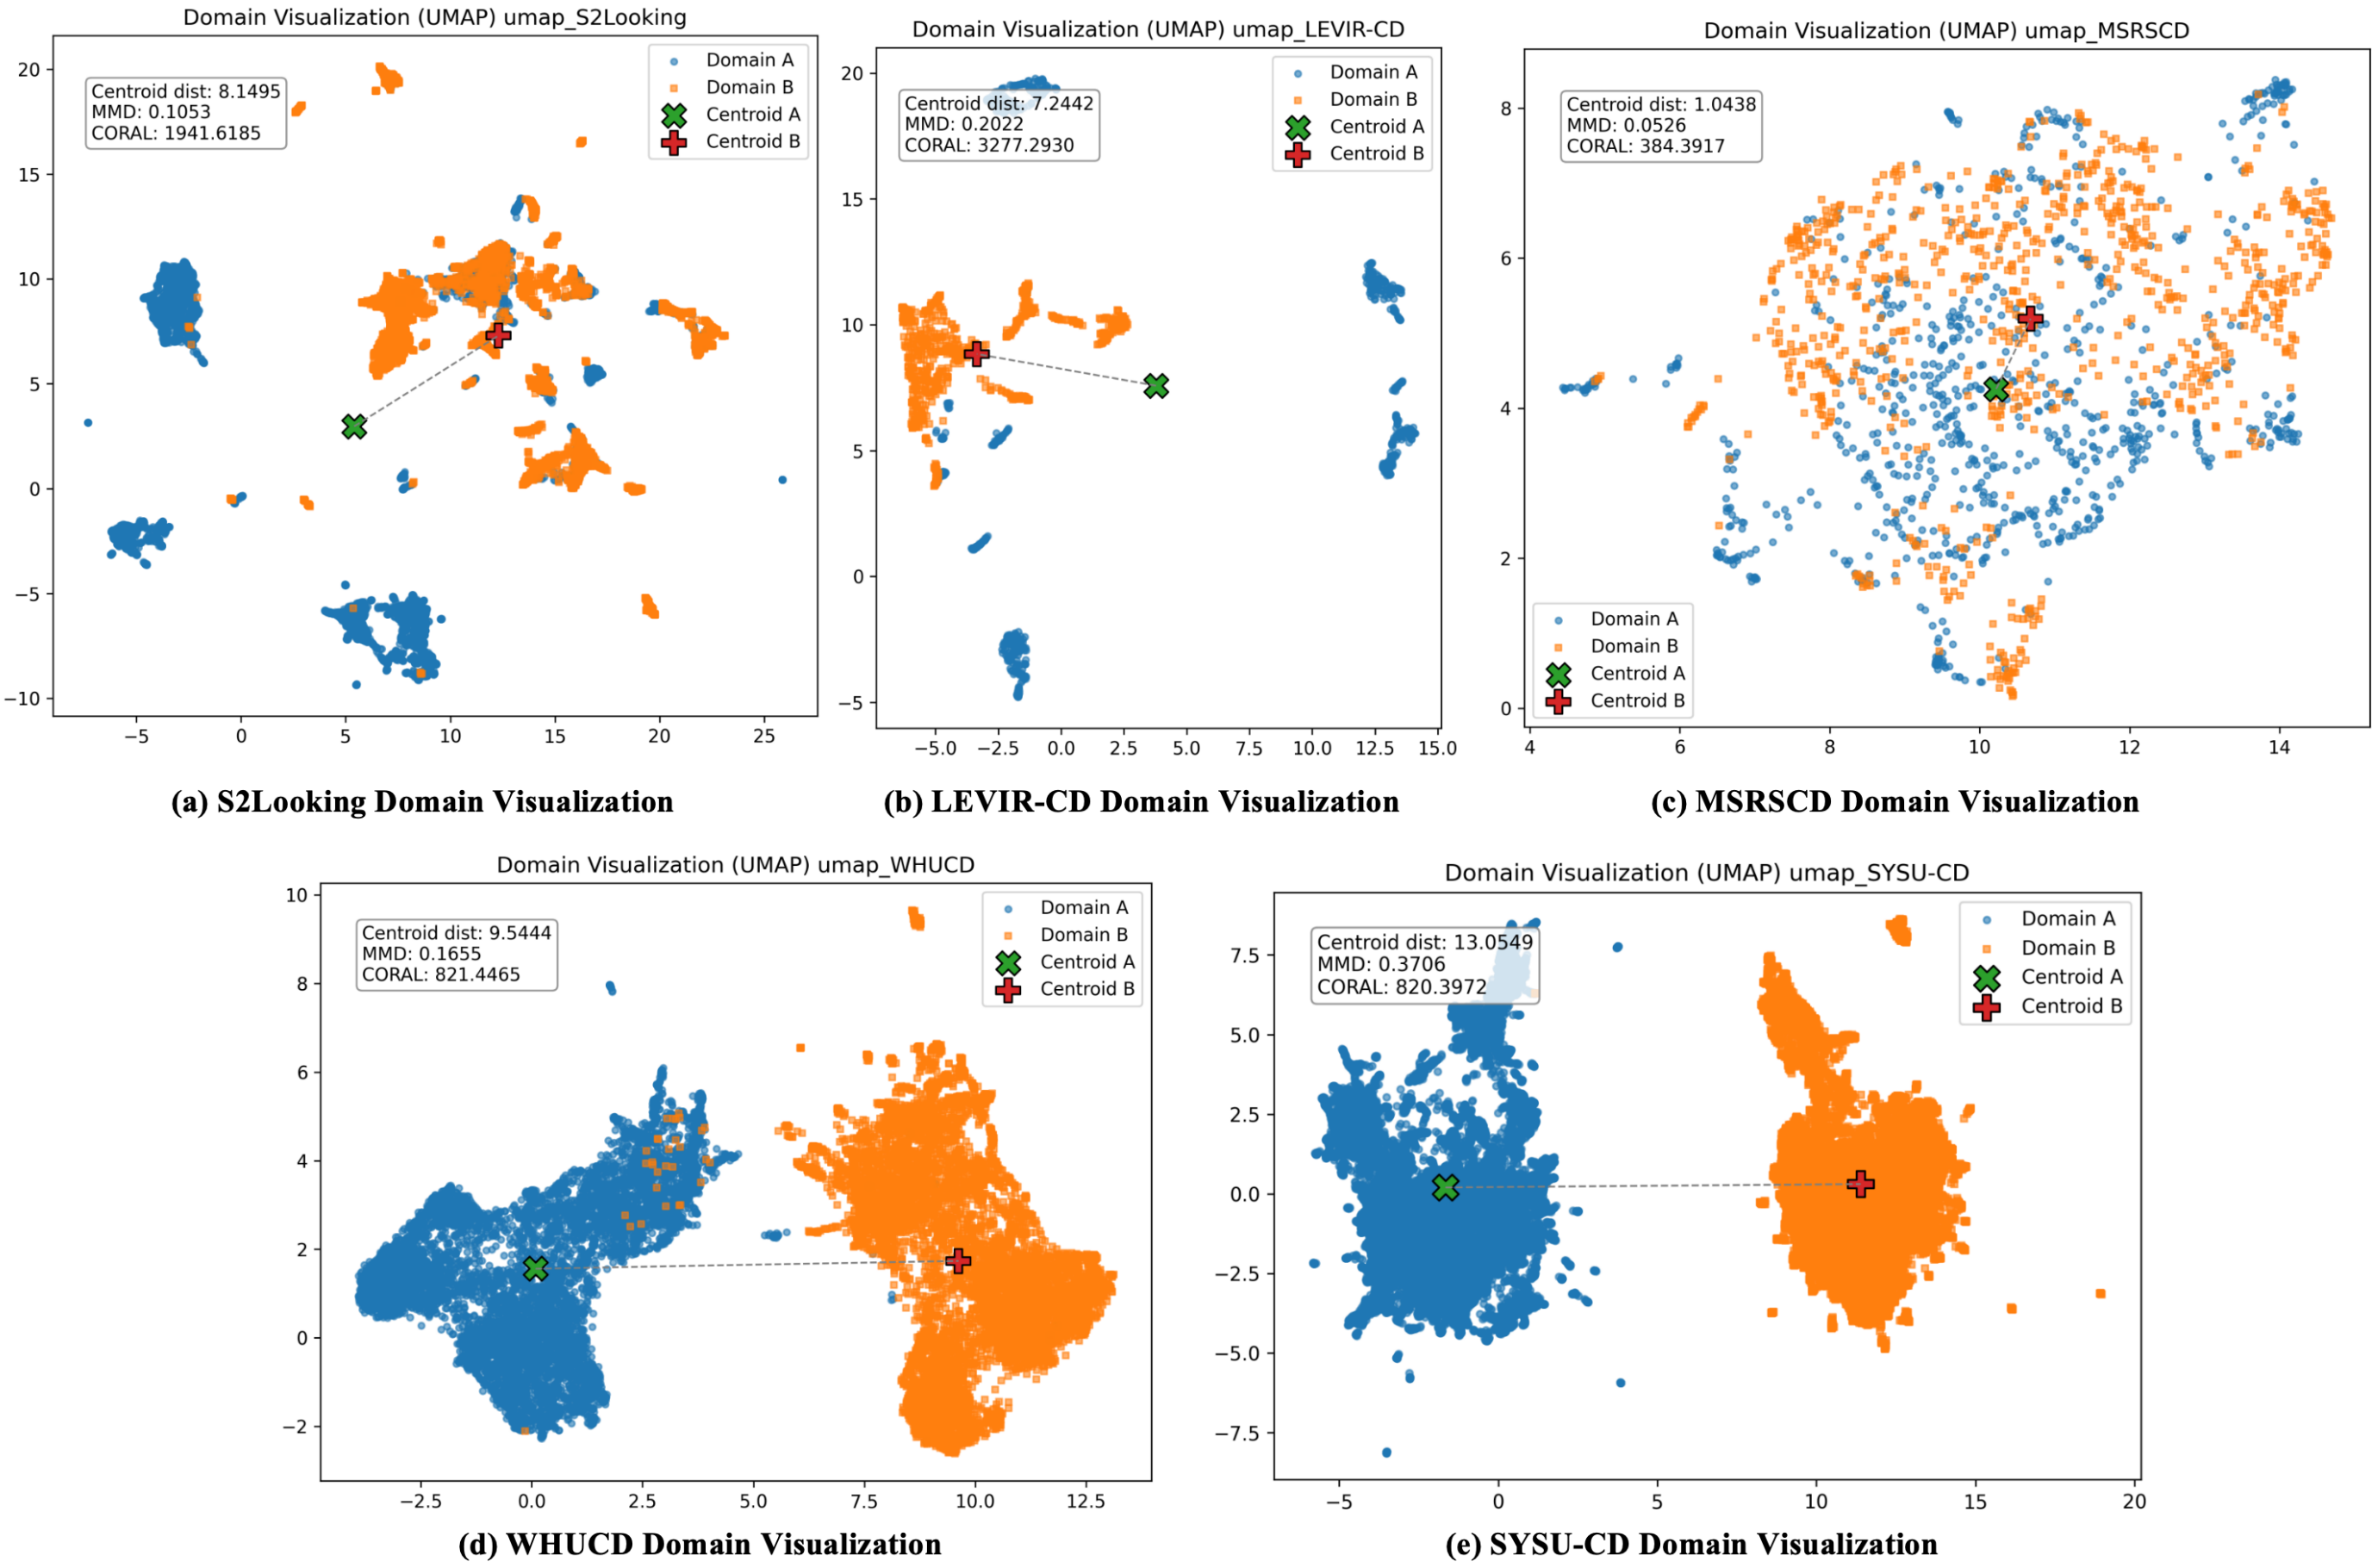
\includegraphics[width=\textwidth]{paper_figures/基于双时相遥感影像风格解缠和内容细化增强遥感变化检测方法/domain_vis.png}
	\caption{该图显示了双时相图像的低级特征经过UMAP投影到二维空间后的分布。圆圈(域A)和方块(域B)代表来自双时相图像的特征样本,标记 \textcolor{green}{\textbf{×}} 和 \textcolor{red}{\textbf{+}} 表示它们各自的质心。连接质心的线表示它们之间的距离,反映了整体域偏移。图中还展示了三个定量域差异度量:质心距离、最大均值差异(MMD)和CORAL距离,它们分别从几何中心、分布一致性和协方差结构的角度表征了域间差异。}
	\label{fig:domain_vis}
\end{figure}



遥感图像特征大致可分为内容特征(代表结构和语义信息,如建筑物、道路)和风格特征(捕获由光照、季节和传感器噪声等因素引起的非结构性差异)。虽然内容是变化检测的核心目标,但风格特征可能引入干扰,从而降低精度。最近的方法,如CCNet~\cite{cheng2024harmony}和DHFF~\cite{jiang2020change},已经探索了内容-风格分离以缓解此问题。然而,大多数现有方法只是简单地移除风格信息,可能忽略了边缘或纹理变化等有益线索。此外,如何有效融合双时相特征以突出变化,同时在复杂场景中保持鲁棒性,仍然是一个未解决的挑战。这些局限性凸显了开发更高效变化检测算法的重大机遇。

为了应对这些挑战,提出了CSDNet,一种新颖的基于CNN的变化检测模型,通过内容-风格分离、细化和特征交互来提高精度和鲁棒性。CSDNet采用HRNet~\cite{Wang2019DeepHR}作为骨干网络,并使用特征金字塔网络(FPN)~\cite{lin_feature_2017}进行多尺度特征融合。本章的主要创新是内容-风格解耦模块(CSDM),它通过实例归一化和门控机制分离并选择性地保留有益的风格特征;以及上下文内容细化模块(Context Content Refinement Module,CCRM)。CCRM位于解码阶段,使用联合通道-空间门控机制进一步细化变化特征,以实现变化区域的精确、细粒度描绘。在五个公共数据集上的实验结果表明,CSDNet显著优于现有最先进的方法,验证了CSDNet在抑制背景干扰和增强差异表示方面的有效性。



综上所述,本章工作的主要贡献如下:

\begin{enumerate}[label=(\arabic*)]
\item 提出了CSDNet,一个通过集成内容-风格分离与通道-空间细化显著改进遥感变化检测的新型模型。
\item 引入了内容-风格解耦模块(CSDM),通过门控机制过滤掉不相关的风格干扰并保留有益的风格线索。
\item 提出了上下文内容细化模块(CCRM),它使用联合通道-空间门控机制来细化特征并增强模型对变化区域的敏感性。
\end{enumerate}

\begin{figure}[!htbp]
	\centering
	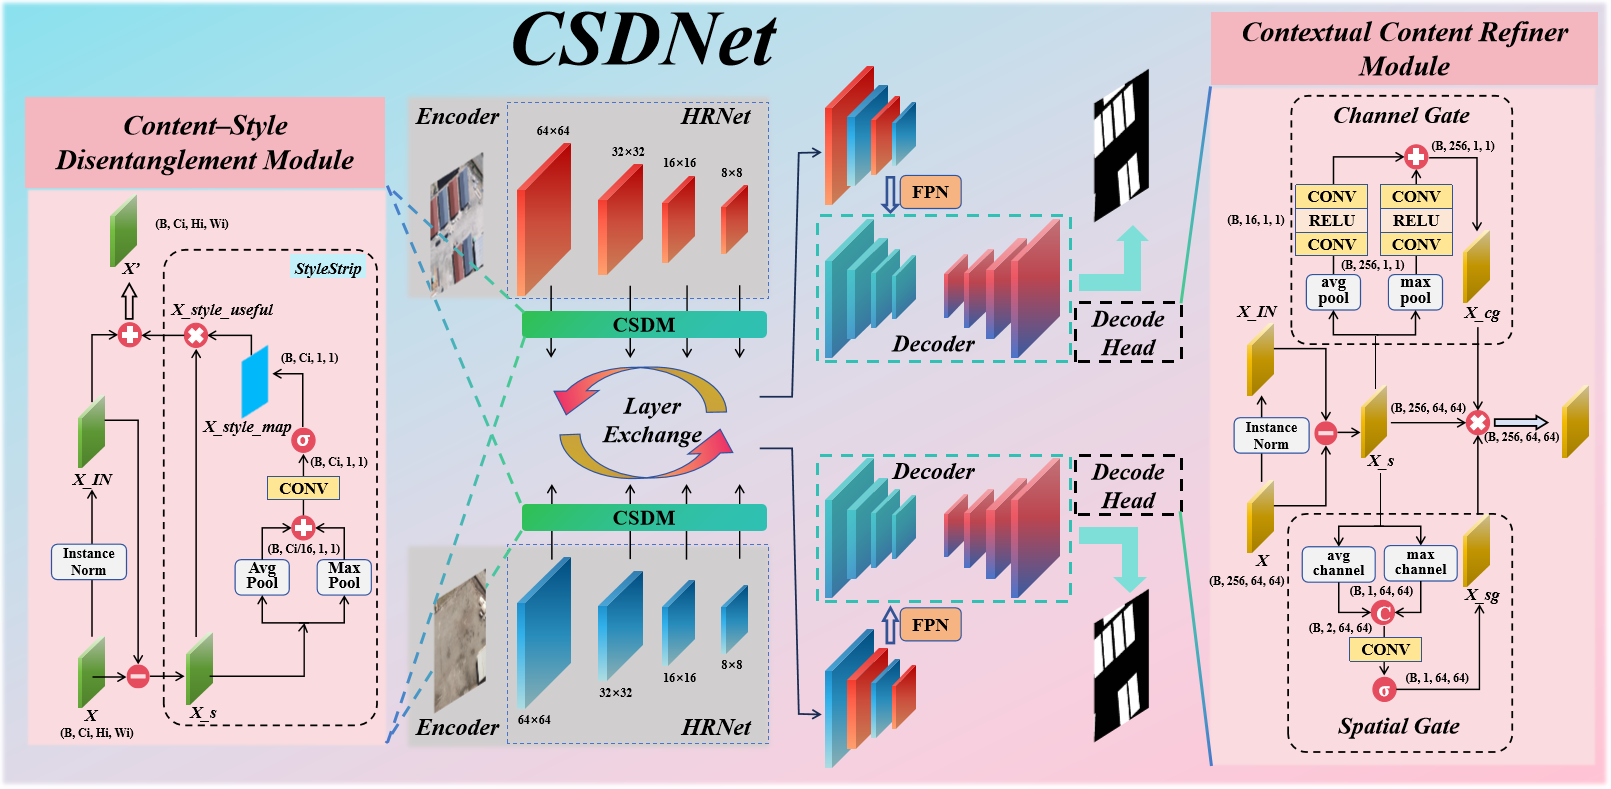
\includegraphics[width=\textwidth]{paper_figures/基于双时相遥感影像风格解缠和内容细化增强遥感变化检测方法/CSDNet.png}
	\caption{CSDNet模型总体结构}
	\label{fig:CSDNet}
\end{figure}



\section{CSDNet模型设计方法}
\subsection{CSDNet总体架构展示}
如图~\ref{fig:CSDNet}所示,模型的整体结构仍旧采用第三章提出的SEED架构。双时相图像首先通过特征提取网络HRNet模型,提取多尺度特征金字塔。随后,特征金字塔通过\textbf{内容-风格解耦模块(CSDM)}进行内容-风格分解,以获得内容特征和风格残差。同时,利用门控机制对风格残差进行过滤,保留对变化检测有用的风格信息,如~\ref{fig:CSDNet}左侧所示。处理后的风格特征随后与原始内容特征重新组合,得到纯化后的特征。在此阶段,使用CSDM模块优化Siamese网络提取的多尺度特征的风格特征,使变化检测模型更专注于提取变化信息,从而优化变化检测任务。

接下来,采用特征层交换机制,对双时相影像的特征金字塔进行跨层交互(参考 EfficientCD~\cite{dong_efficientcd_2024})。具体而言,设时相 $t_1$ 的特征金字塔为 $(F^1_1, F^1_2, F^1_3, F^1_4)$,时相 $t_2$ 的特征金字塔为 $(F^2_1, F^2_2, F^2_3, F^2_4)$,其中下标表示从浅层到深层的金字塔层级。在交换操作中,每隔一层进行特征交换(如 $F^1_2 \leftrightarrow F^2_2$ 和 $F^1_4 \leftrightarrow F^2_4$),从而得到混合金字塔 $(F^1_1, F^2_2, F^1_3, F^2_4)$ 和 $(F^2_1, F^1_2, F^2_3, F^1_4)$。这种方式能够实现跨时相特征的直接对齐,使一个时相的信息注入到另一个时相的非相邻层级,有效提升模型对结构变化的敏感性,同时保持语义层次结构。

随后,基于特征交换后的双时相特征金字塔,使用FPN结构进行特征融合,以获得多尺度双时相特征图。在解码器中,使用常规的逐层上采样进行解码。最后,对于解码头,设计了一个\textbf{上下文内容细化模块(CCRM)},以进一步细化解码器输出的特征,从而增强变化检测的任务相关信号,如图~\ref{fig:CSDNet}右侧所示。细化后的特征随后被映射到变化概率图。在整个CSDNet中,编码器、CSDM、FPN、解码器和解码头等模块均采用参数共享策略,从而实现有效的参数重用,减少模型的参数量。


\subsection{内容风格解缠模块 (CSDM)}
在变化检测任务中,双时相遥感影像采集之间存在显著的时间间隔,这会引入“风格”变化——如大气条件、光照变化和传感器噪声等——这些因素会对孪生神经网络的学习产生不利影响。这些因素在特征层面引入了无关的干扰,从而影响变化检测任务的准确性。为此,设计了内容–风格解耦模块(Content–Style Disentanglement Module, CSDM),如图~\ref{fig:CSDNet}左侧所示。该模块通过“内容–风格”分解和门控机制,选择性地保留对下游任务有益的风格信息,同时剥离冗余部分。对于双时相影像的多尺度特征金字塔,在每个尺度上均采用CSDM模块进行处理。CSDM模块能够显式地将内容信息与风格信息分离,并通过门控机制自适应地选择和保留对变化检测有用的风格特征,使变化检测模型更加专注于变化信息的提取,从而优化变化检测任务。CSDM的计算过程如下:

首先,对输入特征$F\in\mathbb{R}^{C\times H\times W}$应用实例归一化(InstanceNorm)以获得内容特征:
\begin{equation}\label{eq:content}
F_{\mathrm{content}} = \operatorname{IN}(F)
\end{equation}
其中InstanceNorm操作定义为
\begin{equation}
\mu_c = \frac{1}{HW}\sum_{i=1}^{H}\sum_{j=1}^{W}F_{cij},\quad
\sigma_c = \sqrt{\frac{1}{HW}\sum_{i,j}\bigl(F_{cij}-\mu_c\bigr)^2+\epsilon},
\end{equation}
\begin{equation}
\operatorname{IN}(F)_{cij}=\frac{F_{cij}-\mu_c}{\sigma_c},
\end{equation}
该操作将每个样本的每个通道沿空间维度归一化为零均值和单位方差,从而有效地消除了与风格相关的全局统计信息,如亮度、对比度和噪声差异,同时保留了空间结构和局部纹理细节。因此,$\operatorname{IN}(F)$可以被视为图像“内容”信息的有效近似。随后,通过残差计算可以获得输入图像特征的风格残差:
\begin{equation}
F_{\mathrm{style}} = F - F_{\mathrm{content}}
\end{equation}

在GateBlock中,风格残差$F_{\mathrm{style}}\in\mathbb{R}^{C\times H\times W}$首先分别通过全局平均池化和全局最大池化分支进行聚合:
\begin{equation}
A = \mathrm{Conv}_{\mathrm{avg}}\bigl(\mathrm{AvgPool}(F_{\mathrm{style}})\bigr)
\end{equation}
\begin{equation}
\quad\tilde A = \mathrm{ReLU}\bigl(\mathrm{LN}(A)\bigr)
\end{equation}
\begin{equation}
M = \mathrm{Conv}_{\mathrm{max}}\bigl(\mathrm{MaxPool}(F_{\mathrm{style}})\bigr)
\end{equation}
\begin{equation}
\quad\tilde M = \mathrm{ReLU}\bigl(\mathrm{LN}(M)\bigr)
\end{equation}
其中$\mathrm{Conv}_{\mathrm{avg}}$和$\mathrm{Conv}_{\mathrm{max}}$都是用于通道压缩的$1\times1$卷积,$\mathrm{LN}$表示层归一化(LayerNorm)计算,而$\mathrm{ReLU}$是激活函数。随后,将两条路径的特征相加,并通过第二个$1\times1$卷积生成一个通道门控图:
\begin{equation}
S = \tilde A + \tilde M
\end{equation}
\begin{equation}
G = \sigma\bigl(\mathrm{Conv}_2(S)\bigr),\quad G\in[0,1]^{C\times1\times1}
\end{equation}

\begin{equation}
F'_{\mathrm{style}} = F_{\mathrm{style}} \,\otimes\, G
\end{equation}
其中$\mathrm{Conv}_2$是一个将通道扩展回$C$维的$1\times1$卷积,$\sigma$是Sigmoid激活函数,$\otimes$表示逐元素乘法。从上述过程可以看出,CSDM模块使用门控机制对风格残差进行通道加权,从而获得精炼后的风格特征。最后,将剥离出的内容特征与过滤后的风格特征重新组合,得到纯化后的特征:
\begin{equation}
\tilde F = F_{\mathrm{content}} + F'_{\mathrm{style}}
\end{equation}
通过上述计算方法,CSDM使网络能够通过显式剥离和可学习的门控,在去除不相关干扰的同时保留重要的风格线索。这使得网络能够自主学习在何种程度上保留“风格”成分,从而在去噪和信息完整性之间取得平衡。因此,变化检测模型对双时相图像中的风格差异获得了更强的适应性。



\begin{figure}[!htbp]
	\centering
	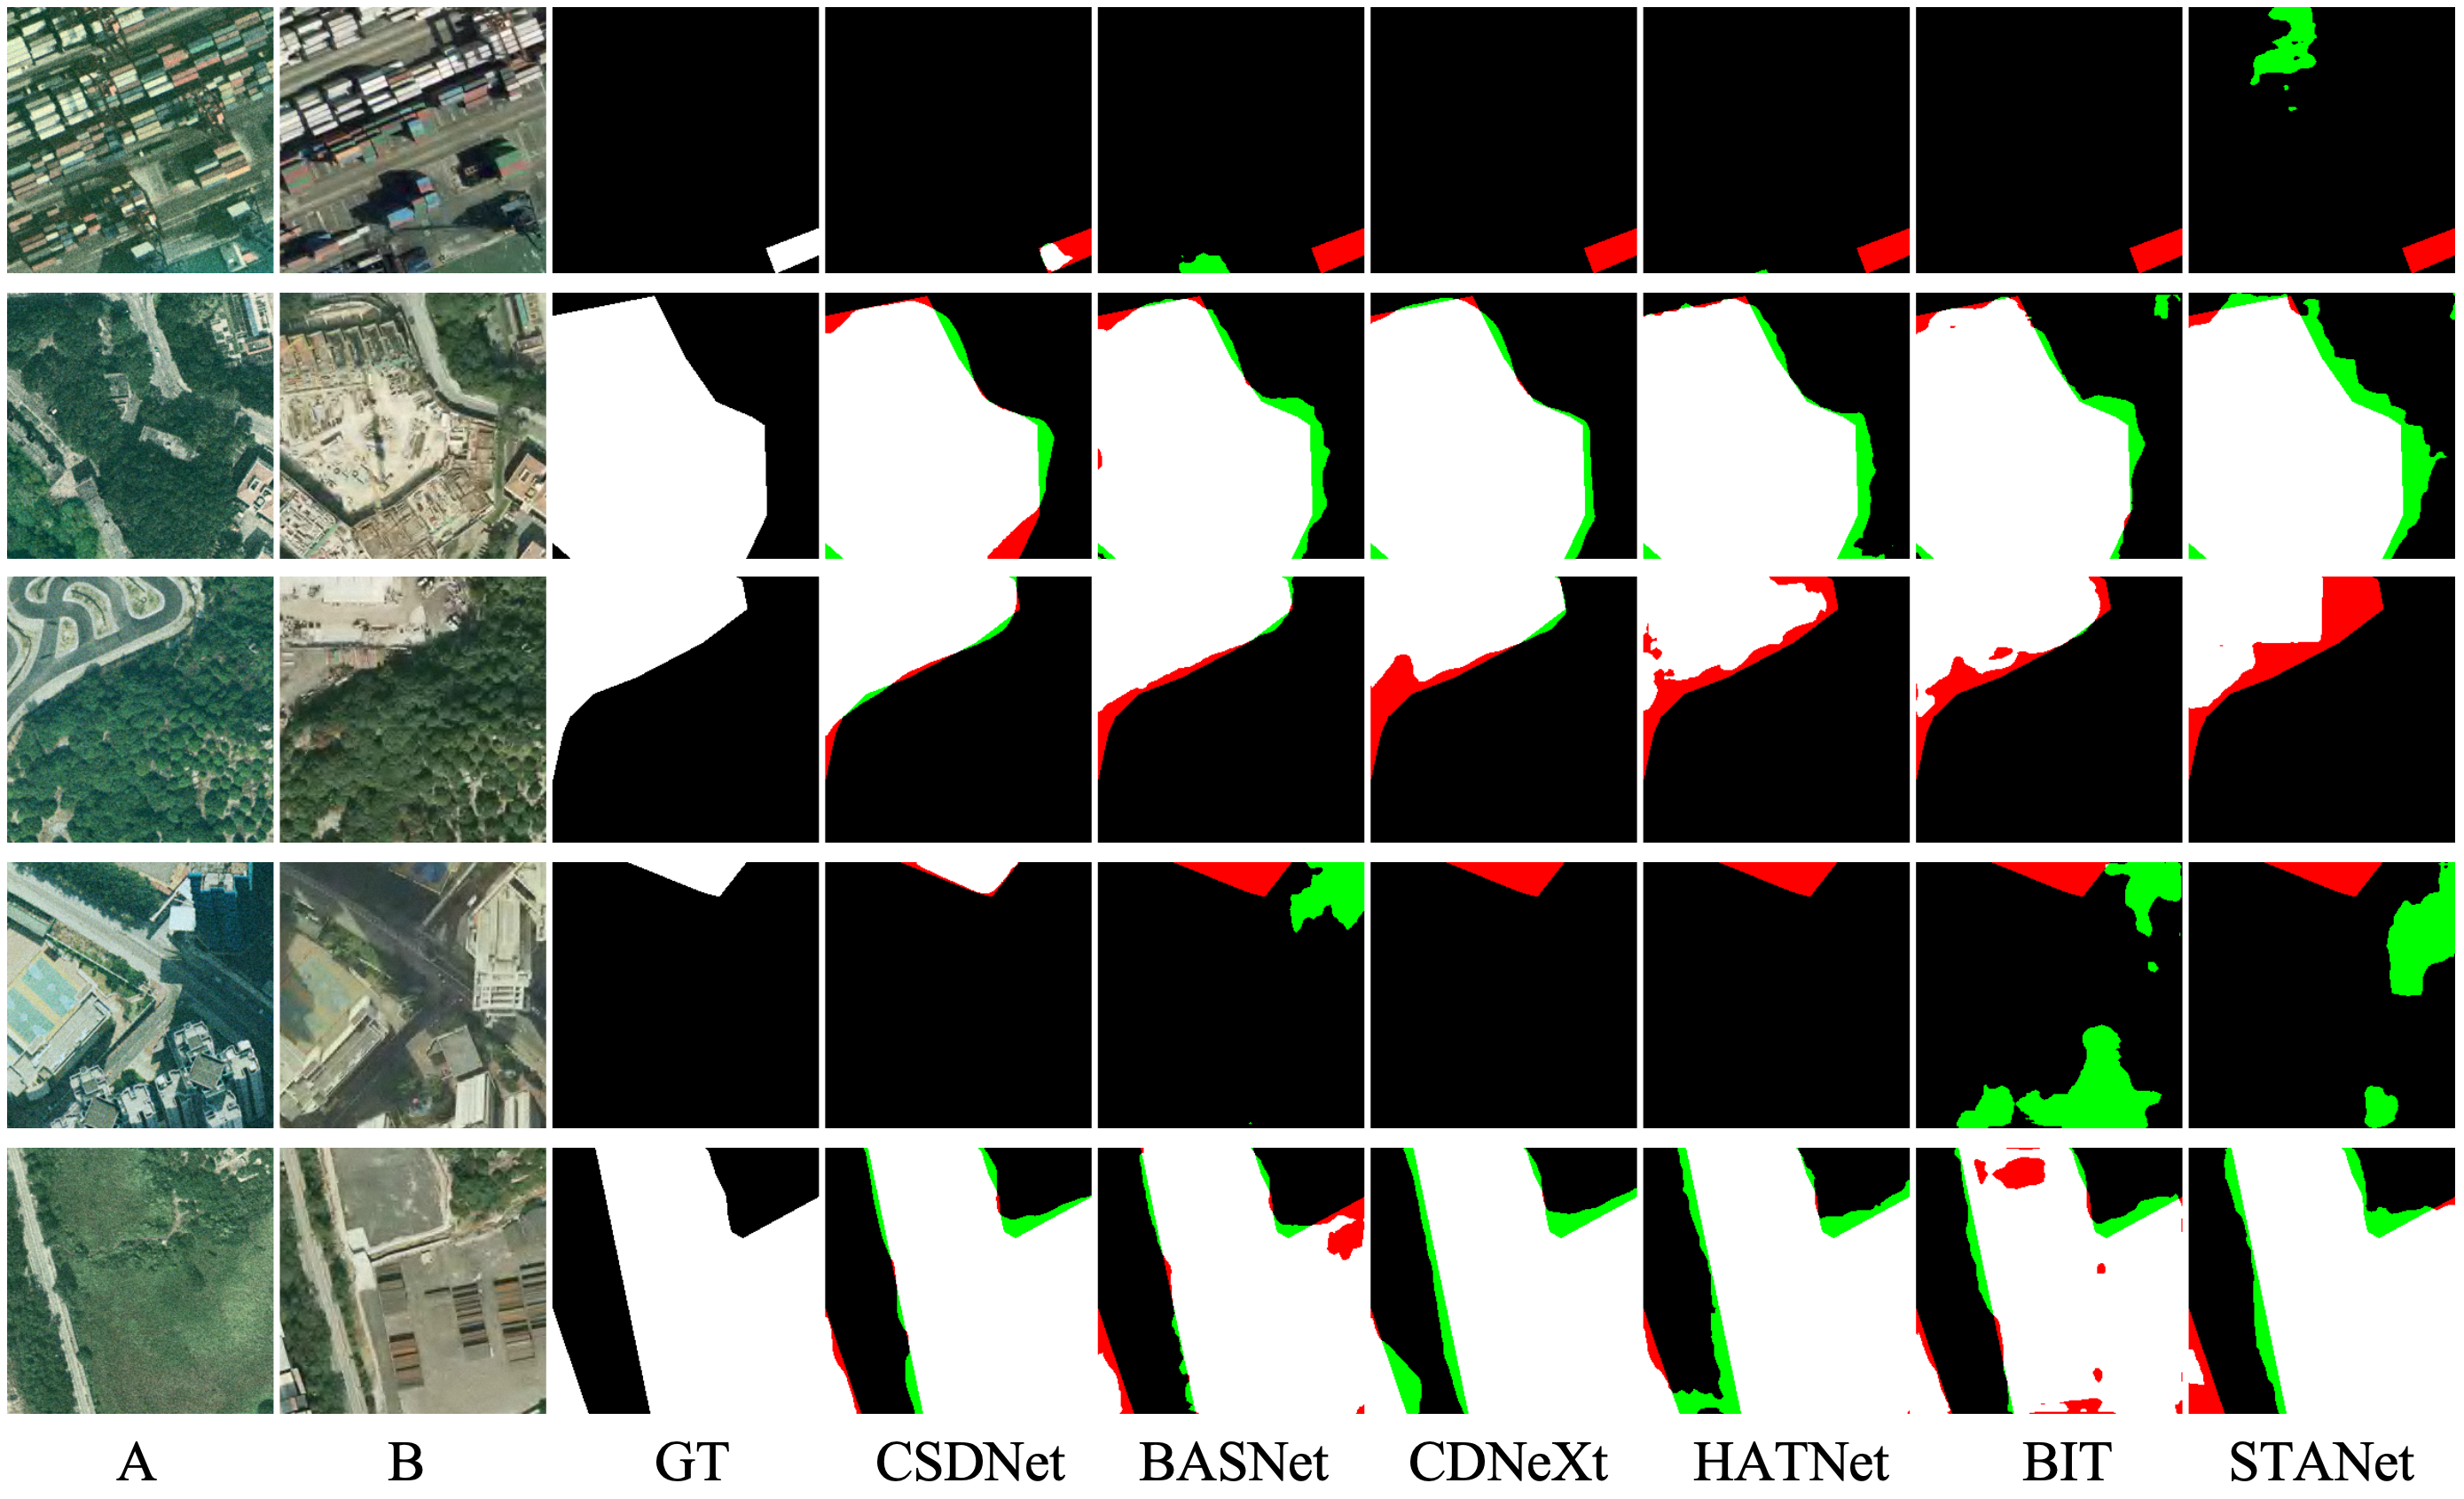
\includegraphics[width=\textwidth]{paper_figures/基于双时相遥感影像风格解缠和内容细化增强遥感变化检测方法/csdnet_sysu.png}
	\caption{CSDNet 模型与经典模型在SYSU-CD测试集上的可视化对比结果}
	\label{fig:csdnet_sysu}
\end{figure}

\begin{table}[!htbp]
\centering
\caption{CSDNet 模型与经典变化检测模型在 SYSU-CD 数据集上的定量对比结果}
\label{tab:csdnet_sysu}
\resizebox{\linewidth}{!}{%
\begin{tabular}{l c c c c c}
\toprule
Method & OA & IoU & F1 & Recall & Precision \\
\midrule
STANet~\cite{chen_spatial-temporal_2020} & 88.24 & 57.22 & 72.79 & 66.71 & 80.08 \\
ISNet~\cite{Cheng2022ISNetTI} & 90.01 & 64.44 & 78.29 & 80.27 & 76.41 \\
BIT~\cite{chen_remote_2022} & 90.64 & 66.03 & 79.54 & 77.13 & 82.10 \\
L-UNet~\cite{Papadomanolaki2021ADM} & 90.58 & 66.15 & 79.63 & 78.08 & 81.24 \\
P2V~\cite{lin_transition_2023} & 90.49 & 66.29 & 79.73 & 79.29 & 80.17 \\
DARNet~\cite{li_densely_2022} & 91.26 & 68.10 & 81.03 & 79.11 & 83.04 \\
SSANet~\cite{Jiang2022JointVL} & -- & 68.18 & 81.08 & 79.73 & 82.48 \\
CDNeXt~\cite{wei_robust_2024} & 91.99 & 68.57 & 81.36 & 74.10 & 90.20 \\
BASNet~\cite{z_wang_bitemporal_2024} & 91.80 & 69.71 & 82.15 & 80.01 & 84.41 \\
HATNet~\cite{Xu2024HybridAT} & 90.92 & 67.00 & 80.24 & 78.23 & 82.36 \\
ChangeCLIP(RN50)~\cite{dong2024changeclip} & 92.08 & 70.53 & 82.72 & 80.41 & 85.16 \\
SGSLN~\cite{zhao_exchanging_2023} & -- & 71.05 & 83.07 & 81.45 & 84.76 \\
ChangeMamba~\cite{chen2024changemamba} & 92.30 & 71.10 & 83.11 & 80.31 & 86.11 \\
\textbf{CSDNet} & 92.39 & 71.16 & 83.15 & 79.60 & 87.03 \\
\bottomrule
\end{tabular}%
}
\end{table}


\subsection{上下文内容细化模块(CCRM)}
在解码器中,对经过逐层上采样和融合后的特征$P\in\mathbb{R}^{C\times H\times W}$引入了上下文内容细化模块(CCRM),以进一步过滤和增强与变化检测任务相关的特征。CCRM包括四个步骤:内容-风格分解、通道门控、空间门控,最后将精炼后的风格重新组合回内容中。

\paragraph{内容-风格分解}
首先,特征图$P$通过实例归一化(InstanceNorm)转换为内容特征$C$,并以残差形式提取风格特征$S$:
\begin{equation}\label{eq:ccr_in}
C = \operatorname{IN}(P),
\end{equation}
\begin{equation}\label{eq:ccr_residual}
S = P - C,
\end{equation}
其中,\(\operatorname{IN}(\cdot)\)在空间上对每个样本的每个通道进行去均值和除以方差的操作,移除了全局统计信息(如亮度、对比度、噪声差异),仅保留纹理和结构信息。这使得\(C\)更加稳定可靠,而\(S\)则包含了剩余的“风格”成分,包括噪声和对变化检测有害的变化。

\paragraph{通道门控}
为了在通道维度上自适应地选择有用的风格成分,CCRM采用了全局平均池化(AvgPool)和全局最大池化(MaxPool)的并行处理,随后通过共享变换生成一个通道门控图\(G_{\mathrm{chan}}\in[0,1]^{C\times1\times1}\)。具体步骤如下:

\begin{equation}\label{eq:ccr_avg_pool}
U_{\mathrm{avg}} = \mathrm{AvgPool}(S), \quad U_{\mathrm{avg}} \in \mathbb{R}^{C\times1\times1}
\end{equation}

\begin{equation}\label{eq:ccr_max_pool}
U_{\mathrm{max}} = \mathrm{MaxPool}(S), \quad U_{\mathrm{max}} \in \mathbb{R}^{C\times1\times1}
\end{equation}

\begin{equation}\label{eq:ccr_fc_avg}
A = W_2\Bigl(\mathrm{ReLU}\bigl(W_1(U_{\mathrm{avg}})\bigr)\Bigr)
\end{equation}

\begin{equation}\label{eq:ccr_fc_max}
M = W_2\Bigl(\mathrm{ReLU}\bigl(W_1(U_{\mathrm{max}})\bigr)\Bigr)
\end{equation}

\begin{equation}\label{eq:ccr_chan_gate}
G_{\mathrm{chan}} = \sigma\bigl(A + M\bigr)
\end{equation}

- 其中$W_1$代表一个通道压缩的$1\times1$卷积,将通道数从$C$减少到$C/r$;经过ReLU激活后,$W_2$使用另一个$1\times1$卷积将通道数恢复到$C$。
- 其中$\sigma$是Sigmoid函数,$G_{\mathrm{chan}}$的每个元素都在$[0,1]$之间,代表相应通道的重要性权重。

通道门控可以根据全局统计信息自适应地抑制或增强特定通道的风格信息,使模型关注于对变化检测有贡献的通道特征。

\paragraph{空间门控}
在空间维度上,首先对风格特征$S$沿通道维度进行平均池化和最大池化,然后将它们拼接起来,并通过一个大感受野的卷积生成一个空间门控图$G_{\mathrm{spat}}\in[0,1]^{1\times H\times W}$:
\begin{equation}\label{eq:ccr_spat_mean}
M_{\mathrm{mean}} = \frac{1}{C}\sum_{c=1}^{C} S_c,\quad M_{\mathrm{mean}}\in\mathbb{R}^{1\times H\times W}
\end{equation}

\begin{equation}\label{eq:ccr_spat_max}
M_{\mathrm{max}} = \max_{c=1,\dots,C} S_c,\quad M_{\mathrm{max}}\in\mathbb{R}^{1\times H\times W}
\end{equation}

\begin{equation}\label{eq:ccr_spat_gate}
G_{\mathrm{spat}} = \sigma\Bigl(\mathrm{Conv}_{7\times7}\bigl([M_{\mathrm{mean}};\,M_{\mathrm{max}}]\bigr)\Bigr)
\end{equation}

- $M_{\mathrm{mean}}$和$M_{\mathrm{max}}$分别捕获了跨通道的平均响应和最强响应。拼接后的双通道输入被送入一个$7\times7$卷积以获得丰富的空间上下文。

\paragraph{风格重组与输出}
最后,通道门控和空间门控都作用于$S$,其结果被加回到内容特征$C$中,以获得精炼后的特征$\hat P$:
\begin{equation}\label{eq:ccr_style_refine}
S' = S \otimes G_{\mathrm{chan}} \otimes G_{\mathrm{spat}},
\end{equation}
\begin{equation}\label{eq:ccr_output}
\hat P = C + S'.
\end{equation}

\noindent
这里,\(\hat P\)是精炼后的特征图,包含了经过门控过滤的风格信息。通过这种方式,CCRM可以在通道和空间两个维度上自适应地过滤风格信息,抑制不相关的干扰,并保留对变化检测有帮助的特征,从而显著提高解码器输出的语义准确性和鲁棒性。


\begin{figure}[!htbp]
	\centering
	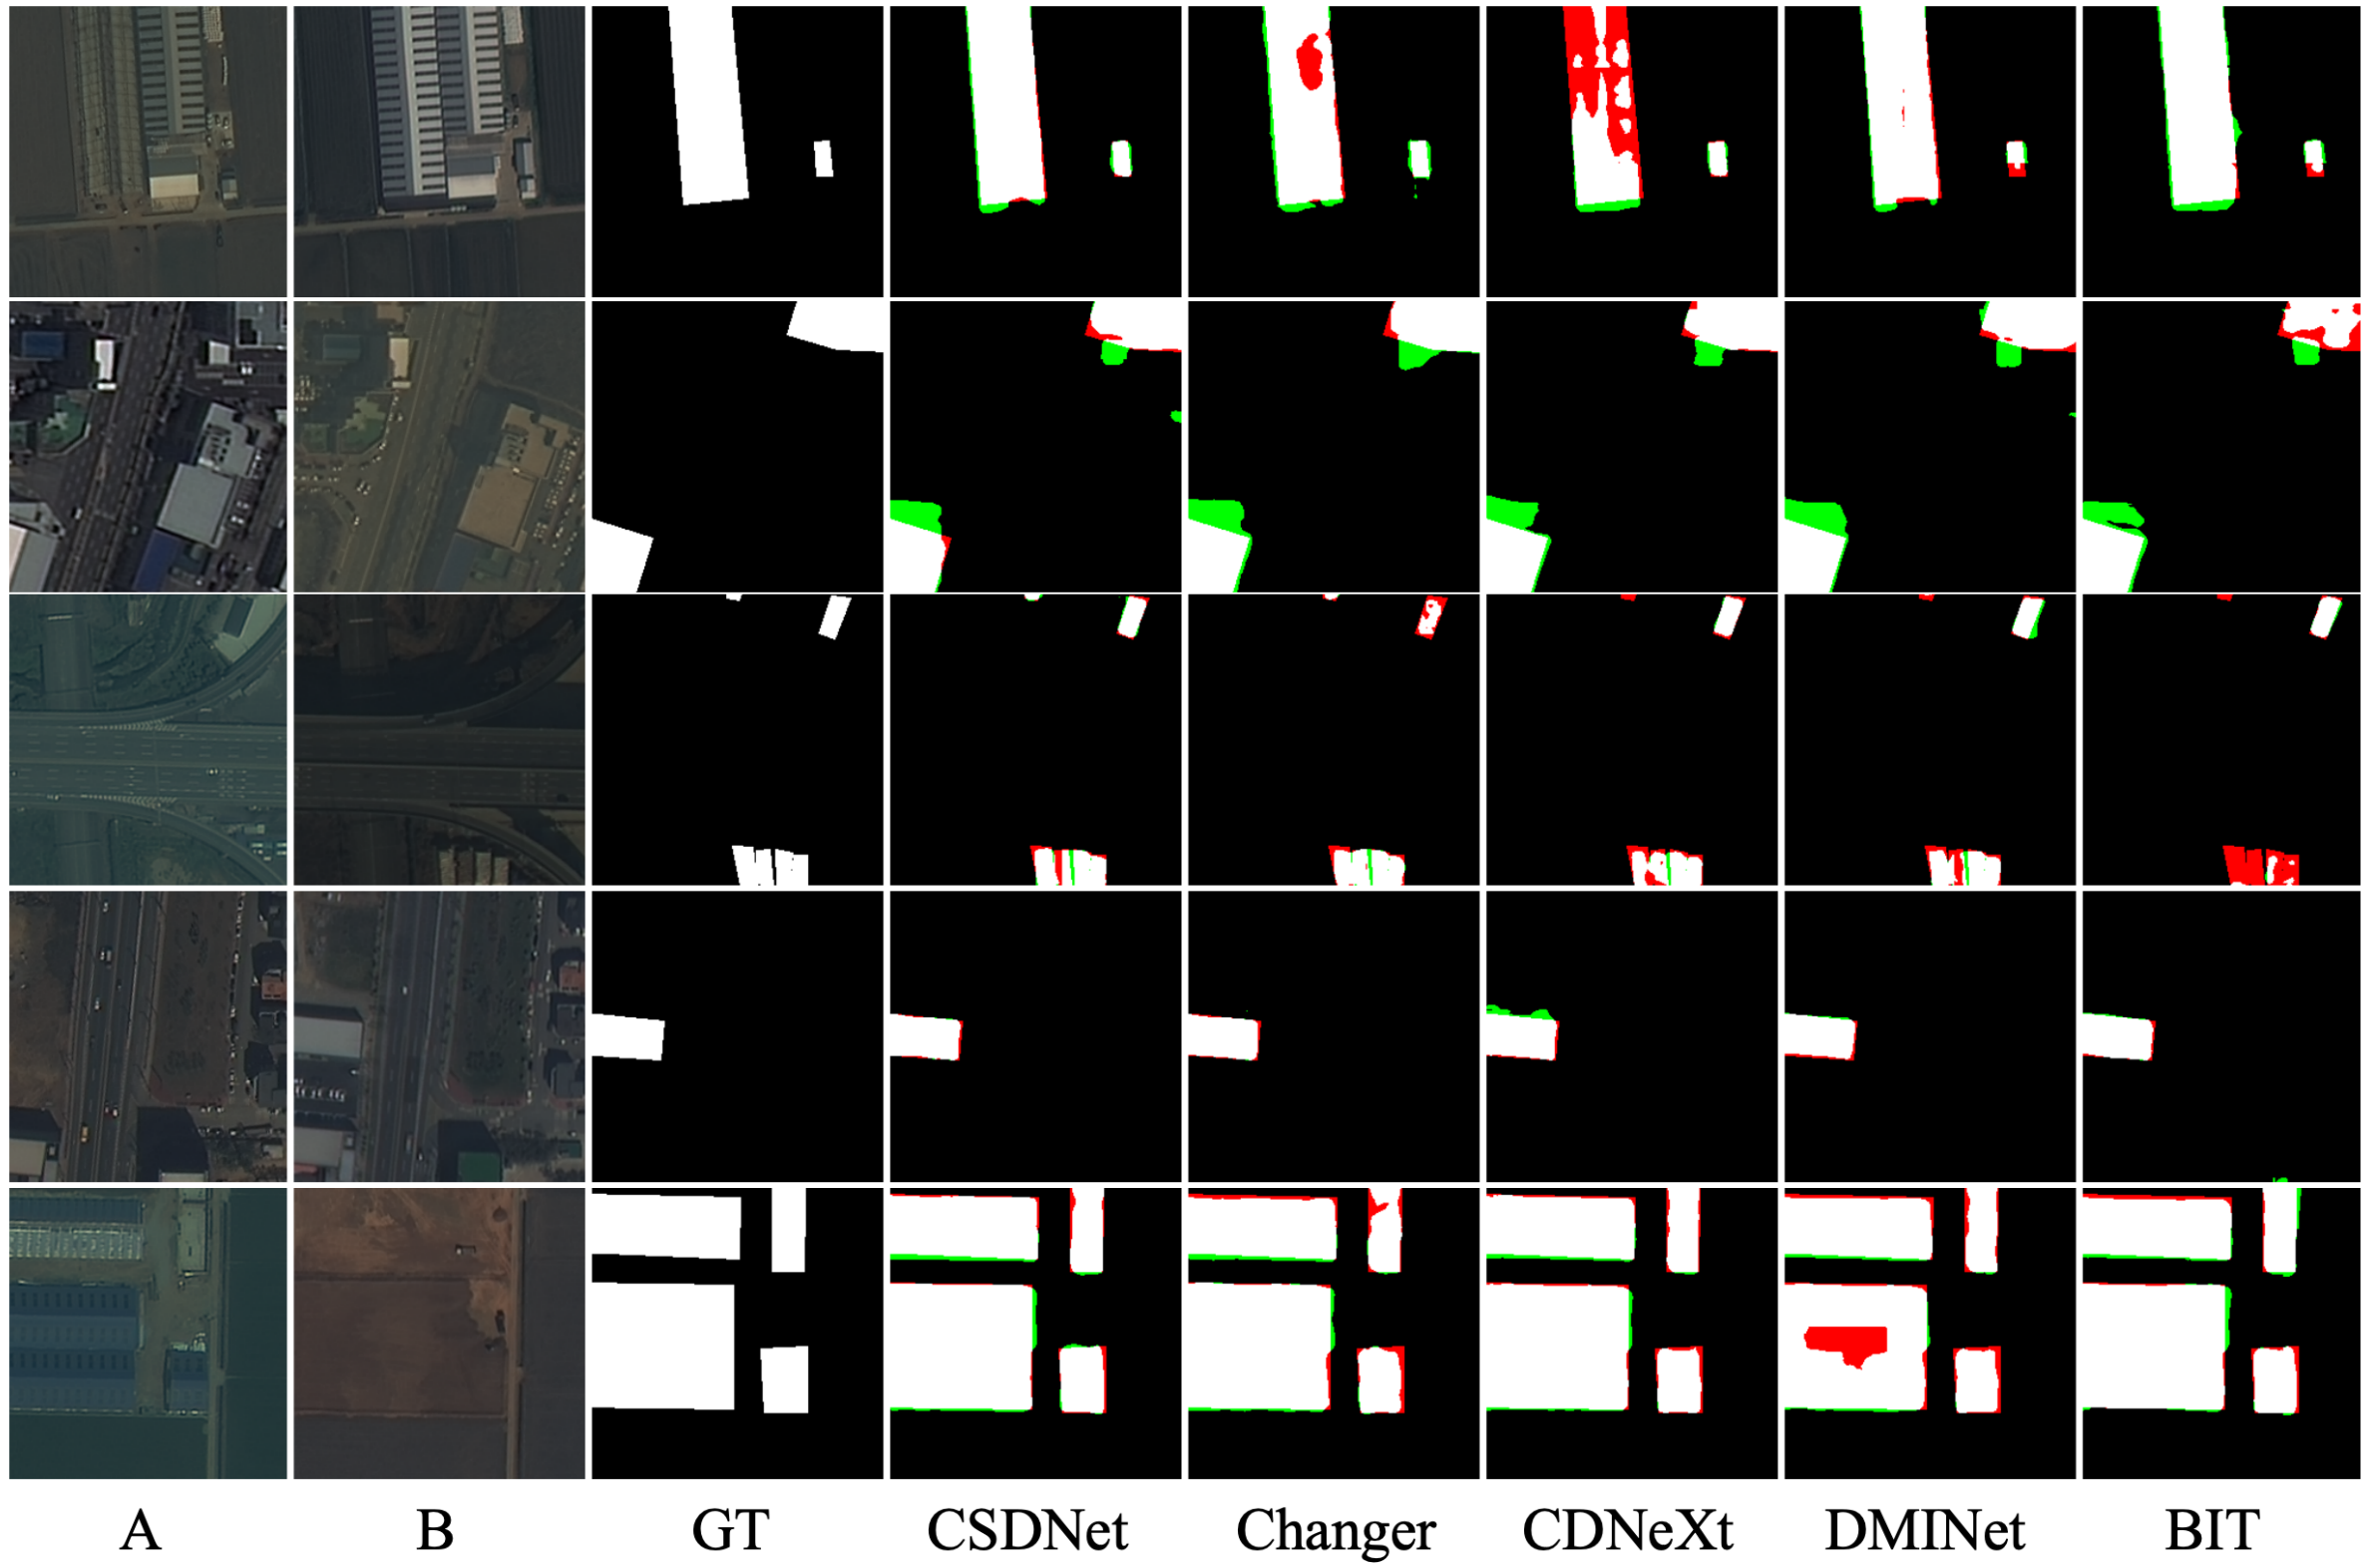
\includegraphics[width=\textwidth]{paper_figures/基于双时相遥感影像风格解缠和内容细化增强遥感变化检测方法/csdnet_s2looking.png}
	\caption{CSDNet 模型与经典模型在S2Looking测试集上的可视化对比结果}
	\label{fig:csdnet_s2looking}
\end{figure}

\begin{table}[!htbp]
\centering
\caption{模型与经典变化检测模型在 S2Looking 数据集上的定量对比结果}
\label{tab:csdnet_s2looking}
\resizebox{\linewidth}{!}{%
\begin{tabular}{l c c c c c}
\toprule
Method & OA & IoU & F1 & Recall & Precision \\
\midrule
HATNet~\cite{Xu2024HybridAT} & -- & 47.08 & 64.02 & 60.90 & 67.48 \\
FHD~\cite{Pei2022FeatureHD} & -- & 47.33 & 64.25 & 56.71 & 74.09 \\
CGNet~\cite{han_change_2023} & -- & 47.41 & 64.33 & 59.38 & 70.18 \\
BIT~\cite{chen_remote_2022} & 99.24 & 47.94 & 64.81 & 58.15 & 73.20 \\
SAM-CD~\cite{ding2024adapting} & -- & 48.29 & 65.13 & 58.92 & 72.80 \\
DMINet~\cite{feng_change_2023} & 99.20 & 48.33 & 65.16 & 62.13 & 68.51 \\
PCAANet~\cite{Xu2023ProgressiveCA} & 99.22 & 48.54 & 65.36 & 61.54 & 69.68 \\
HFIFNet~\cite{Han2025HFIFNetHF} & 99.22 & 48.54 & 65.35 & 61.04 & 70.33 \\
CDNeXt~\cite{wei_robust_2024} & -- & 50.05 & 66.71 & 63.08 & 70.78 \\
Changer~\cite{Fang2022ChangerFI} & -- & 50.47 & 67.08 & 62.04 & 73.01 \\
\textbf{CSDNet} & 99.24 & 50.72 & 67.31 & 64.34 & 70.55 \\
\bottomrule
\end{tabular}%
}
\end{table}

\subsection{CSDNet中的损失函数}
在CSDNet模型中,使用一种基于交叉熵的简单损失函数来训练模型。如~\ref{fig:CSDNet}所示,有两个等效的解码头(Decode Head)。该模型采用双分支二元分类方案,并使用交叉熵进行监督。设两个分支的原始logit为\(o^{(1)}\)和\(o^{(2)}\),真实标签为\(y\in\{0,1\}\)。单个分支的交叉熵损失定义为
\begin{equation}
\mathcal{L}_{\mathrm{CE}}(o, y)
= -\log\left(\frac{\exp(o_{y})}{\sum_{k=0}^1 \exp(o_{k})}\right),
\end{equation}
其中\(o_k\)表示对应于类别\(k\)的logit。在训练期间,最终的损失是两个分支级交叉熵损失的平均值:
\begin{equation}
\mathcal{L}_{\text{train}}
= \frac{1}{2}\left(\mathcal{L}_{\mathrm{CE}}\bigl(o^{(1)}, y\bigr)
+ \mathcal{L}_{\mathrm{CE}}\bigl(o^{(2)}, y\bigr)\right).
\end{equation}
这种形式利用了两个分支之间的冗余性和互补性来提高鲁棒性,而平均操作则防止了任何单个分支主导梯度。在推理时,将两个分支的logit进行平均以产生最终预测:
\begin{equation}
\hat{o} = \frac{1}{2}\left(o^{(1)} + o^{(2)}\right),
\end{equation}
与使用单个分支相比,这会产生更平滑、更稳定的分类输出。

\section{实验结果与分析}

\begin{figure}[!htbp]
	\centering
	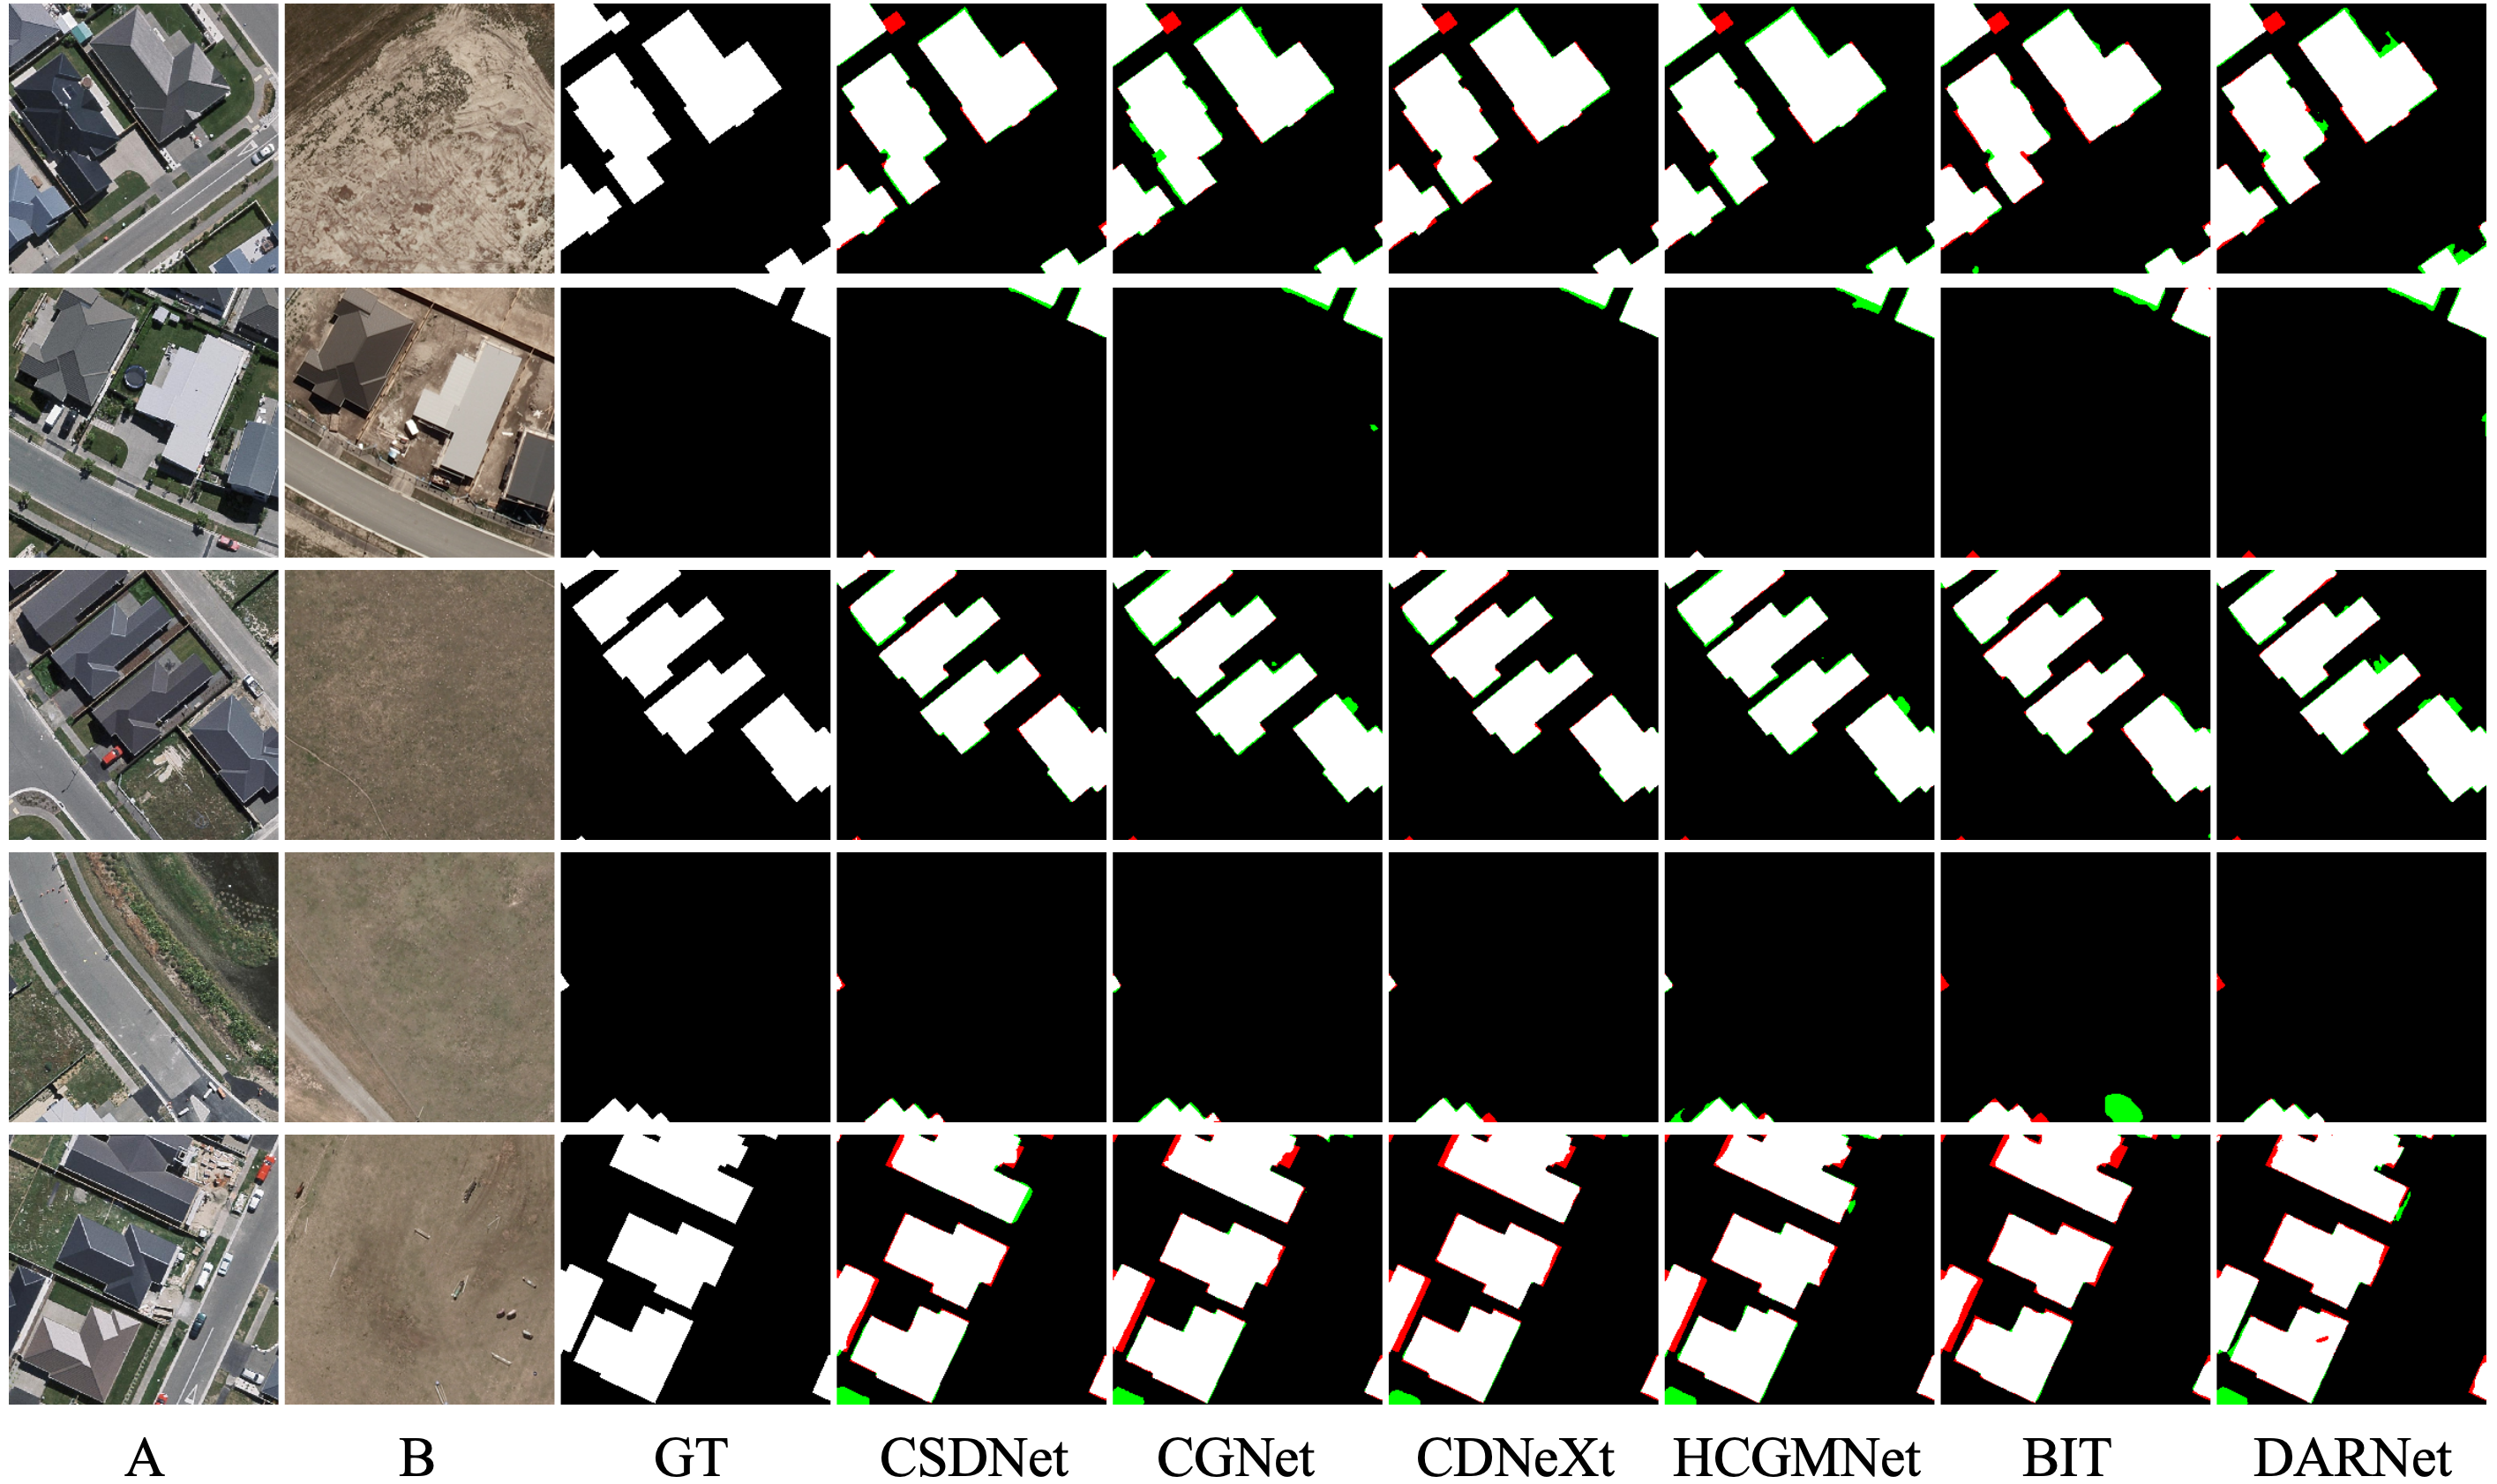
\includegraphics[width=\linewidth]{paper_figures/基于双时相遥感影像风格解缠和内容细化增强遥感变化检测方法/csdnet_whucd.png}
    \caption{CSDNet 模型与经典模型在 WHUCD 测试集上的可视化对比结果}
	\label{fig:csdnet_whucd}
\end{figure}

\begin{table}[!htbp]
\centering
\caption{CSDNet 模型与经典变化检测模型在 WHUCD 数据集上的定量对比结果}
\label{tab:csdnet_whucd}
\resizebox{\linewidth}{!}{%
\begin{tabular}{l c c c c c}
\toprule
Method & OA & IoU & F1 & Recall & Precision \\
\midrule
CDNet~\cite{Alcantarilla2016StreetviewCD} & 98.96 & 79.59 & 88.63 & 87.24 & 90.07 \\
ISDANet~\cite{h_ren_interactive_2025} & 99.05 & 82.26 & 90.27 & 94.84 & 86.12 \\
DARNet~\cite{li_densely_2022} & 99.19 & 83.92 & 91.26 & 91.71 & 90.82 \\
SNUNet~\cite{Fang2021SNUNetCDAD} & 99.24 & 84.69 & 91.71 & 90.77 & 92.67 \\
P2V~\cite{lin_transition_2023} & 99.31 & 85.91 & 92.42 & 90.93 & 93.97 \\
DSIFN~\cite{Zhang2020ADS} & 99.34 & 86.36 & 92.68 & 90.20 & 95.30 \\
MSCANet~\cite{m_liu_cnn-transformer_2022} & 99.36 & 86.65 & 92.85 & 89.98 & 95.90 \\
SGSLN~\cite{zhao_exchanging_2023} & 99.38 & 87.47 & 93.32 & 92.91 & 93.72 \\
BIT~\cite{chen_remote_2022} & 99.43 & 88.22 & 93.74 & 92.00 & 95.56 \\
HCGMNet~\cite{Han2023HCGMNetAH} & 99.52 & 90.10 & 94.79 & 95.31 & 94.27 \\
ChangeCLIP(RN50)~\cite{dong2024changeclip} & 99.52 & 90.15 & 94.82 & 94.02 & 95.63 \\
CDNeXt~\cite{wei_robust_2024} & 99.54 & 90.35 & 94.93 & 92.56 & 97.43 \\
CGNet~\cite{han_change_2023} & 99.54 & 90.41 & 94.96 & 94.61 & 95.32 \\
EfficientCD~\cite{dong_efficientcd_2024} & 99.55 & 90.71 & 95.13 & 94.19 & 96.08 \\
SAFDNet~\cite{Fu2025BeyondCD} & 99.55 & 90.73 & 95.14 & 94.47 & 95.82 \\
\textbf{CSDNet} & 99.56 & 90.88 & 95.22 & 95.12 & 95.33 \\
\bottomrule
\end{tabular}%
}
\end{table}


\begin{figure}[!htbp]
	\centering
	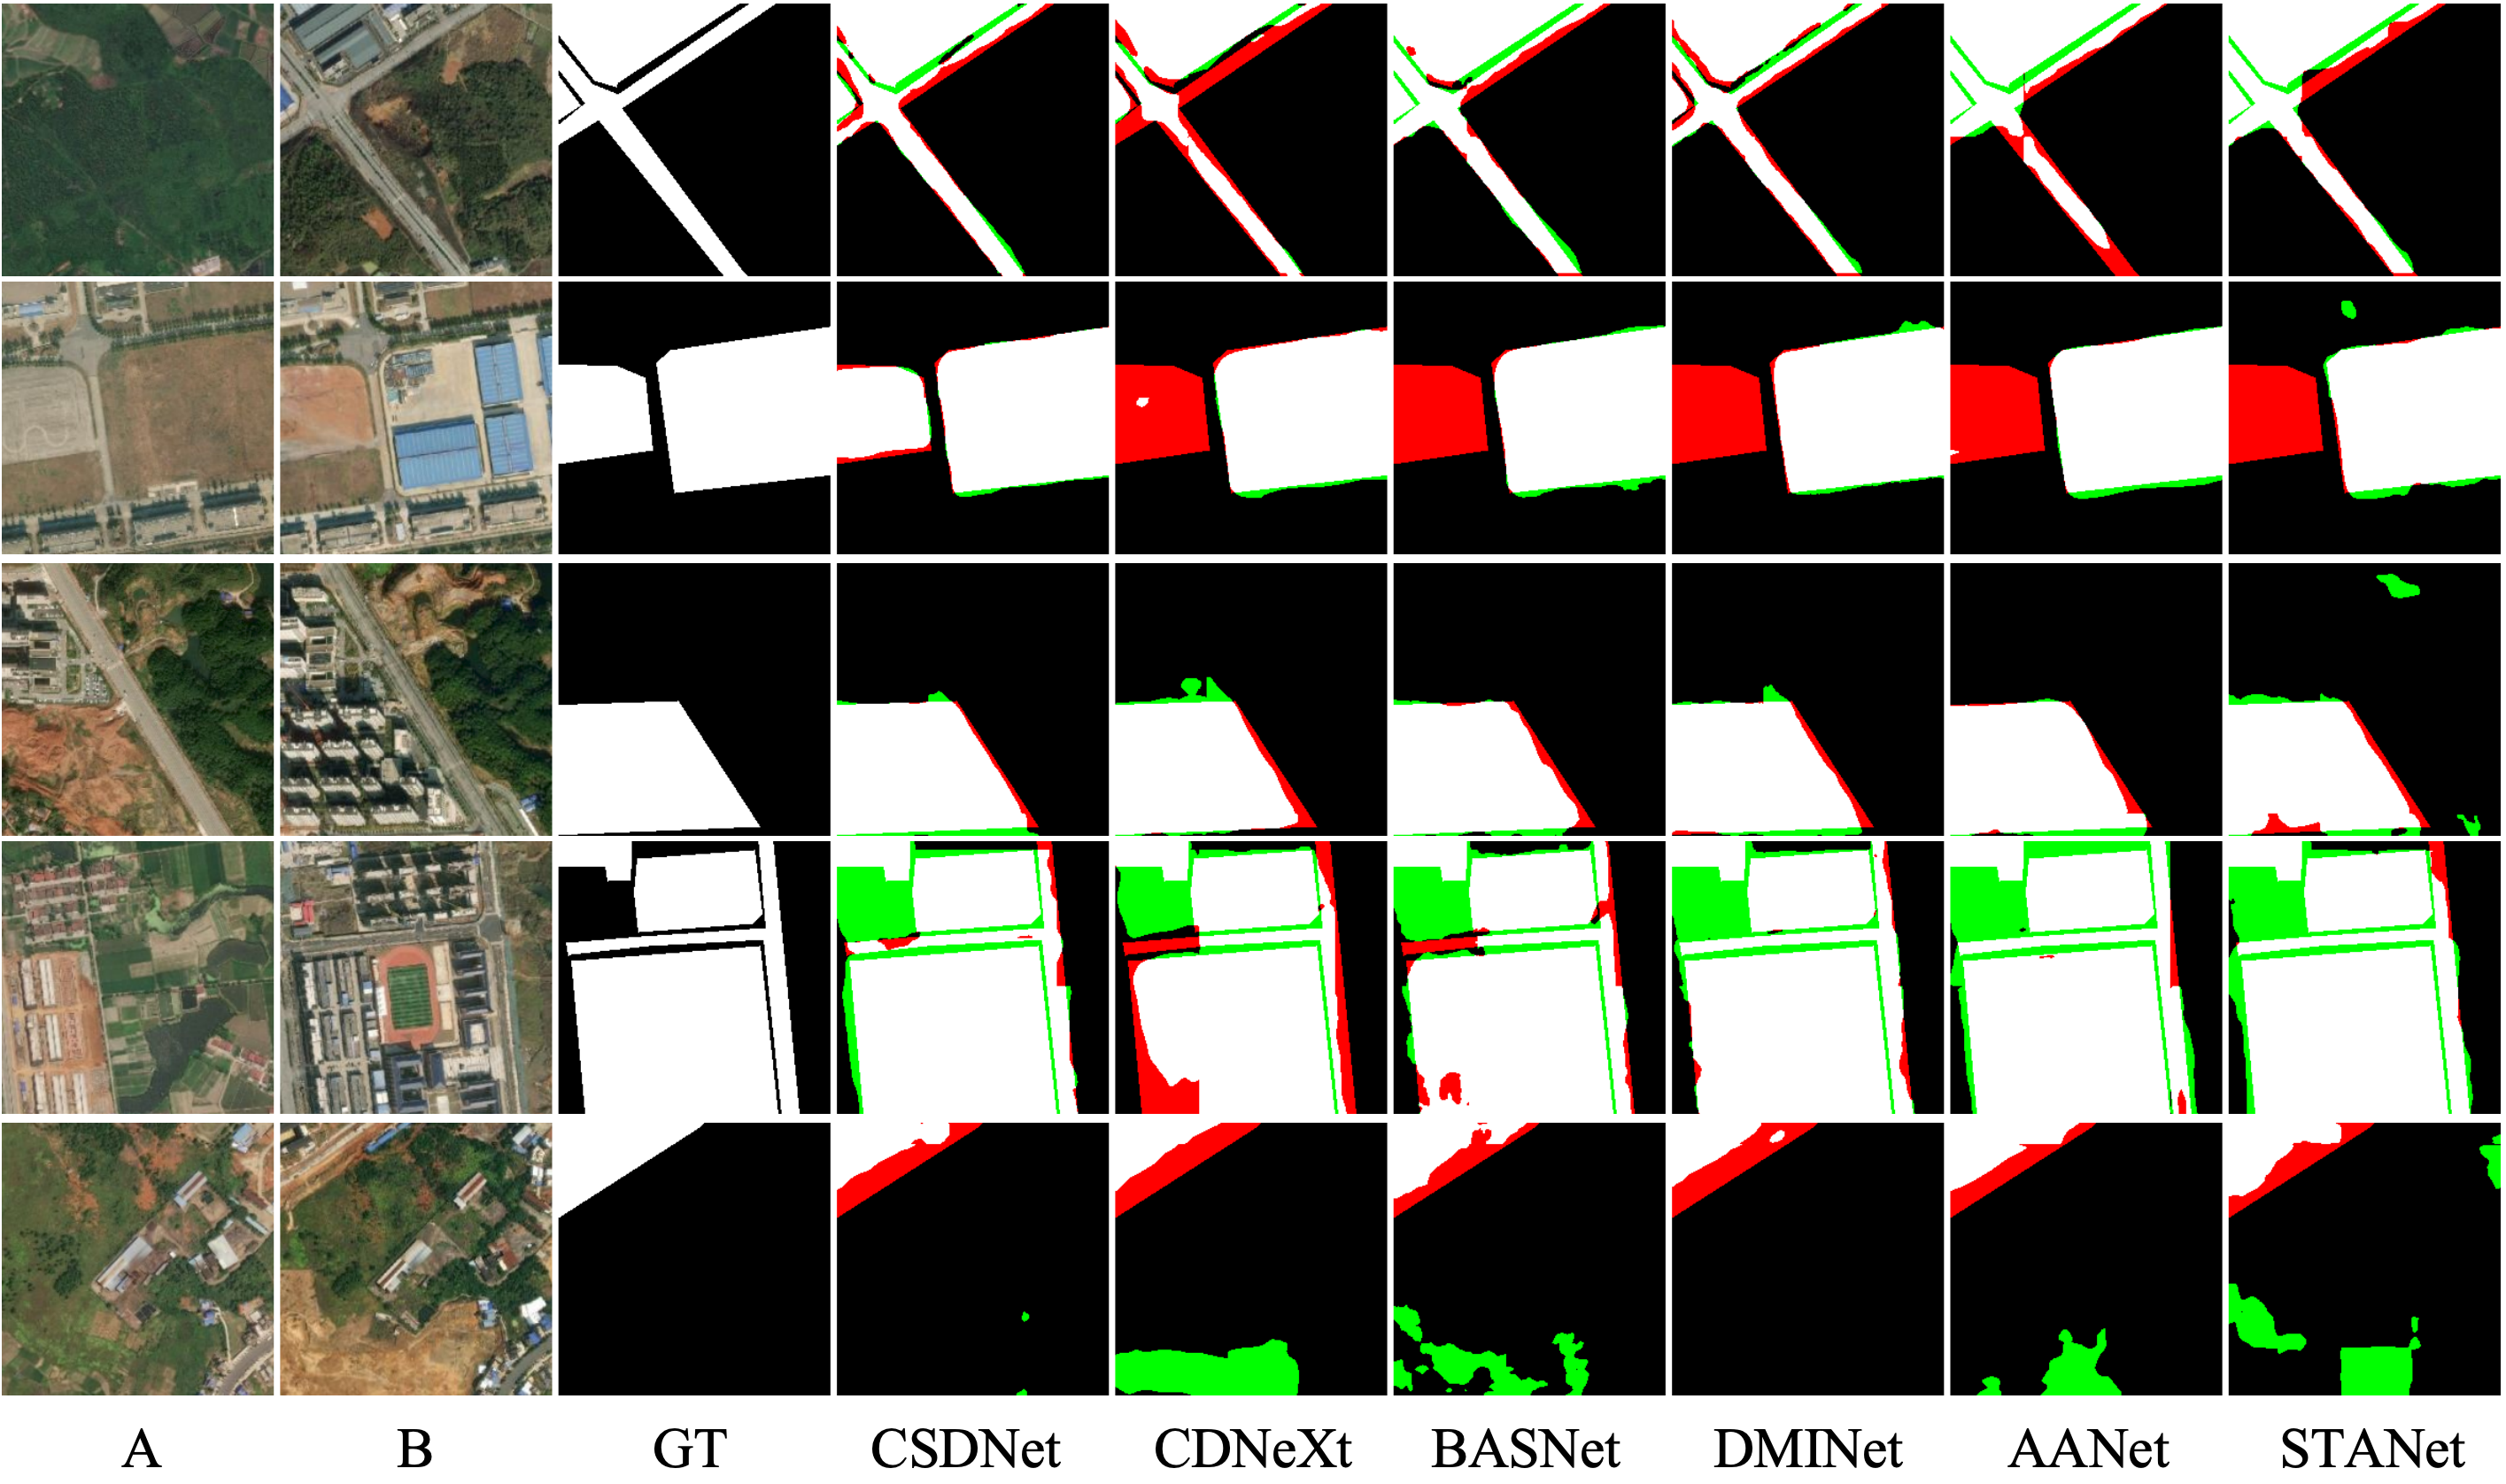
\includegraphics[width=\linewidth]{paper_figures/基于双时相遥感影像风格解缠和内容细化增强遥感变化检测方法/csdnet_msrscd.png}
    \caption{CSDNet 模型与经典模型在 MSRSCD 测试集上的可视化对比结果}
	\label{fig:csdnet_msrscd}
\end{figure}

\subsection{定量分析与可视化结果}

\begin{table}[!htbp]
\centering
\caption{CSDNet 模型与经典模型在 MSRSCD 数据集上的定量对比结果}
\label{tab:csdnet_msrscd}
\resizebox{\linewidth}{!}{%
\begin{tabular}{l c c c c c}
\toprule
Method & OA & IoU & F1 & Recall & Precision \\
\midrule
STANet~\cite{chen_spatial-temporal_2020} & 91.44 & 54.52 & 70.57 & 69.46 & 71.71 \\
SGSLN~\cite{zhao_exchanging_2023} & 92.52 & 56.28 & 73.36 & 69.73 & 77.39 \\
ChangeFormer~\cite{bandara2022transformer} & 91.86 & 56.96 & 72.58 & 72.94 & 72.22 \\
FCCDN~\cite{Chen2021FCCDNFC} & 92.36 & 57.94 & 73.37 & 71.30 & 75.56 \\
AANet~\cite{Hang2024AANetAA} & 92.17 & 59.23 & 74.40 & 77.03 & 71.94 \\
EATDer~\cite{Ma2024EATDerEA} & 91.47 & 59.29 & 74.44 & 84.17 & 66.73 \\
MSNet~\cite{Liu2025NetworkAD} & 93.03 & 59.80 & 75.74 & 74.73 & 76.79 \\
DMINet~\cite{feng_change_2023} & 93.05 & 61.24 & 75.96 & 74.37 & 77.63 \\
BASNet~\cite{z_wang_bitemporal_2024} & 92.87 & 61.31 & 76.02 & 76.51 & 75.53 \\
CDNeXt~\cite{wei_robust_2024} & 93.24 & 61.59 & 76.23 & 73.42 & 79.27 \\
DFFNet~\cite{Liu2025FullScaleCD} & 93.23 & 61.82 & 77.44 & 78.69 & 76.22 \\
\textbf{CSDNet} & 93.07 & 62.01 & 76.55 & 76.38 & 76.73 \\
\bottomrule
\end{tabular}%
}
\end{table}

\subsection{实验结果量化指标与可视化分析}

如表~\ref{tab:csdnet_sysu}、表~\ref{tab:csdnet_s2looking}、表~\ref{tab:csdnet_whucd}、表~\ref{tab:csdnet_msrscd} 和表~\ref{tab:csdnet_levir} 所示,在五个广泛使用的遥感变化检测数据集上对 CSDNet 进行了评估,并将其性能与代表性的 SOTA方法进行了比较。总体而言,CSDNet 取得了一致具有竞争力或更优的结果,在 SYSU-CD、S2Looking、WHUCD 和 MSRSCD 数据集上优势明显,特别是在 IoU 和 F1 分数方面。这些性能提升归功于 CSDM 和 CCRM 模块,它们有效地解耦并精炼了内容-风格特征,使模型能够在复杂场景中更好地捕捉有意义的变化。

在 SYSU-CD 数据集上,CSDNet 达到了最高的 IoU (71.16) 和 F1 分数 (83.15),超过了 ChangeMamba 和 CDNeXt 等强基线模型。这表明,即使在竞争方法已经达到很高精度的情况下,内容-风格精炼策略仍然能带来可观的收益。对于具有显著视角变化和光照差异的 S2Looking 数据集,CSDNet 获得了 50.72 的 IoU,比先前的最佳方法 (Changer) 高出 0.25。这证明了风格分离与精炼策略在具有挑战性的跨域条件下提高了模型的鲁棒性。在 WHUCD 数据集上,许多方法的性能已接近饱和,但 CSDNet 仍然取得了最佳的 IoU (90.88),并保持了平衡的精度 (Precision, 95.33) 和召回率 (Recall, 95.12),突显了其在保留精细结构细节的同时避免对噪声过拟合的能力。对于 MSRSCD 数据集,CSDNet 略微超过了先前的 SOTA 方法,取得了最高的 IoU (62.01),并与 DFFNet 等多尺度精炼基线相比,展现了更稳定的召回率-精度权衡。这表明 CSDM 中的通道-空间联合门控机制和 CCRM 中的跨尺度精炼有助于在不同背景复杂度的场景下保持准确检测。在 LEVIR-CD 数据集上,CSDNet 取得了有竞争力的结果,其性能接近现有的最佳方法,表明CSDNet在大型建筑变化检测任务中依然有效,尽管相较于顶级基线模型没有显著的提升。

图~\ref{fig:csdnet_sysu}、图~\ref{fig:csdnet_s2looking}、图~\ref{fig:csdnet_whucd}、图~\ref{fig:csdnet_msrscd} 和 图~\ref{fig:csdnet_levir} 展示了在 SYSU-CD、S2Looking、WHUCD 和 MSRSCD 数据集上的定性比较结果。为了便于直观理解,不同颜色分别代表真阳性 (TP, 白色)、假阳性 (FP, 红色)、真阴性 (TN, 黑色) 和假阴性 (FN, 绿色)。在具有复杂地表覆盖变化的挑战性样本中,CSDNet 产生的假阳性和假阴性少于其他方法,并且其边界定位在小尺度变化上尤为准确,这在 SYSU-CD 和 WHUCD 数据集上可以观察到。像 HATNet 和 STANet 等模型表现出更频繁的假阳性,而 CDNeXt 则偶尔会漏掉细微的变化。这些观察结果与定量分析一致,证实了 CSDNet 能有效抑制不相关的风格噪声,并强调与变化相关的结构信息。


\subsection{CSDNet 消融实验分析}

为了验证所提出的内容-风格解耦模块 (Content–Style Disentanglement Module, CSDM) 和上下文内容精炼模块 (Contextual Content Refiner Module, CCRM) 的有效性,进行了一系列消融实验,在 SYSU-CD、LEVIR-CD、WHUCD、MSRSCD 和 S2Looking 五个公开数据集上,以 IoU 为主要评估指标,评估了模型在不同配置下的性能。如表~\ref{tab:csdnet_ablation} 所示,当模型不包含 CSDM 和 CCRM 模块作为基线时,其在各个数据集上的 IoU 表现处于基础水平。令人鼓舞的是,当独立引入 CSDM 模块后,模型在所有数据集上的性能均得到显著提升。这有力地证明了 CSDM 通过其内容-风格解耦机制,有效抑制了背景风格噪声,增强了双时相图像间的特征对齐,从而提高了模型感知真实变化的能力,在处理具有复杂或异构风格差异的图像时表现出尤为突出的鲁棒性。同样地,在独立引入 CCRM 模块后,模型性能也呈现出积极的提升。这验证了 CCRM 在解码阶段,能够通过上下文内容精炼和联合通道-空间门控机制对特征进行再提纯,增强了对变化区域的感知,并有助于更精细地描绘变化区域。最重要的是,当 CSDM 和 CCRM 模块被同时集成时,模型的性能达到了最佳状态,在所有数据集上均取得了最高的 IoU。这强有力地证明了 CSDM 和 CCRM 并非简单的叠加效应,而是在编码和解码阶段通过有效的协同工作,共同提升了模型的特征表示能力和变化检测性能。CSDM 在前期处理风格噪声、提纯特征,而 CCRM 则在后期对这些提纯后的特征进行更精细的上下文感知精炼。


\begin{figure}[!htbp]
	\centering
	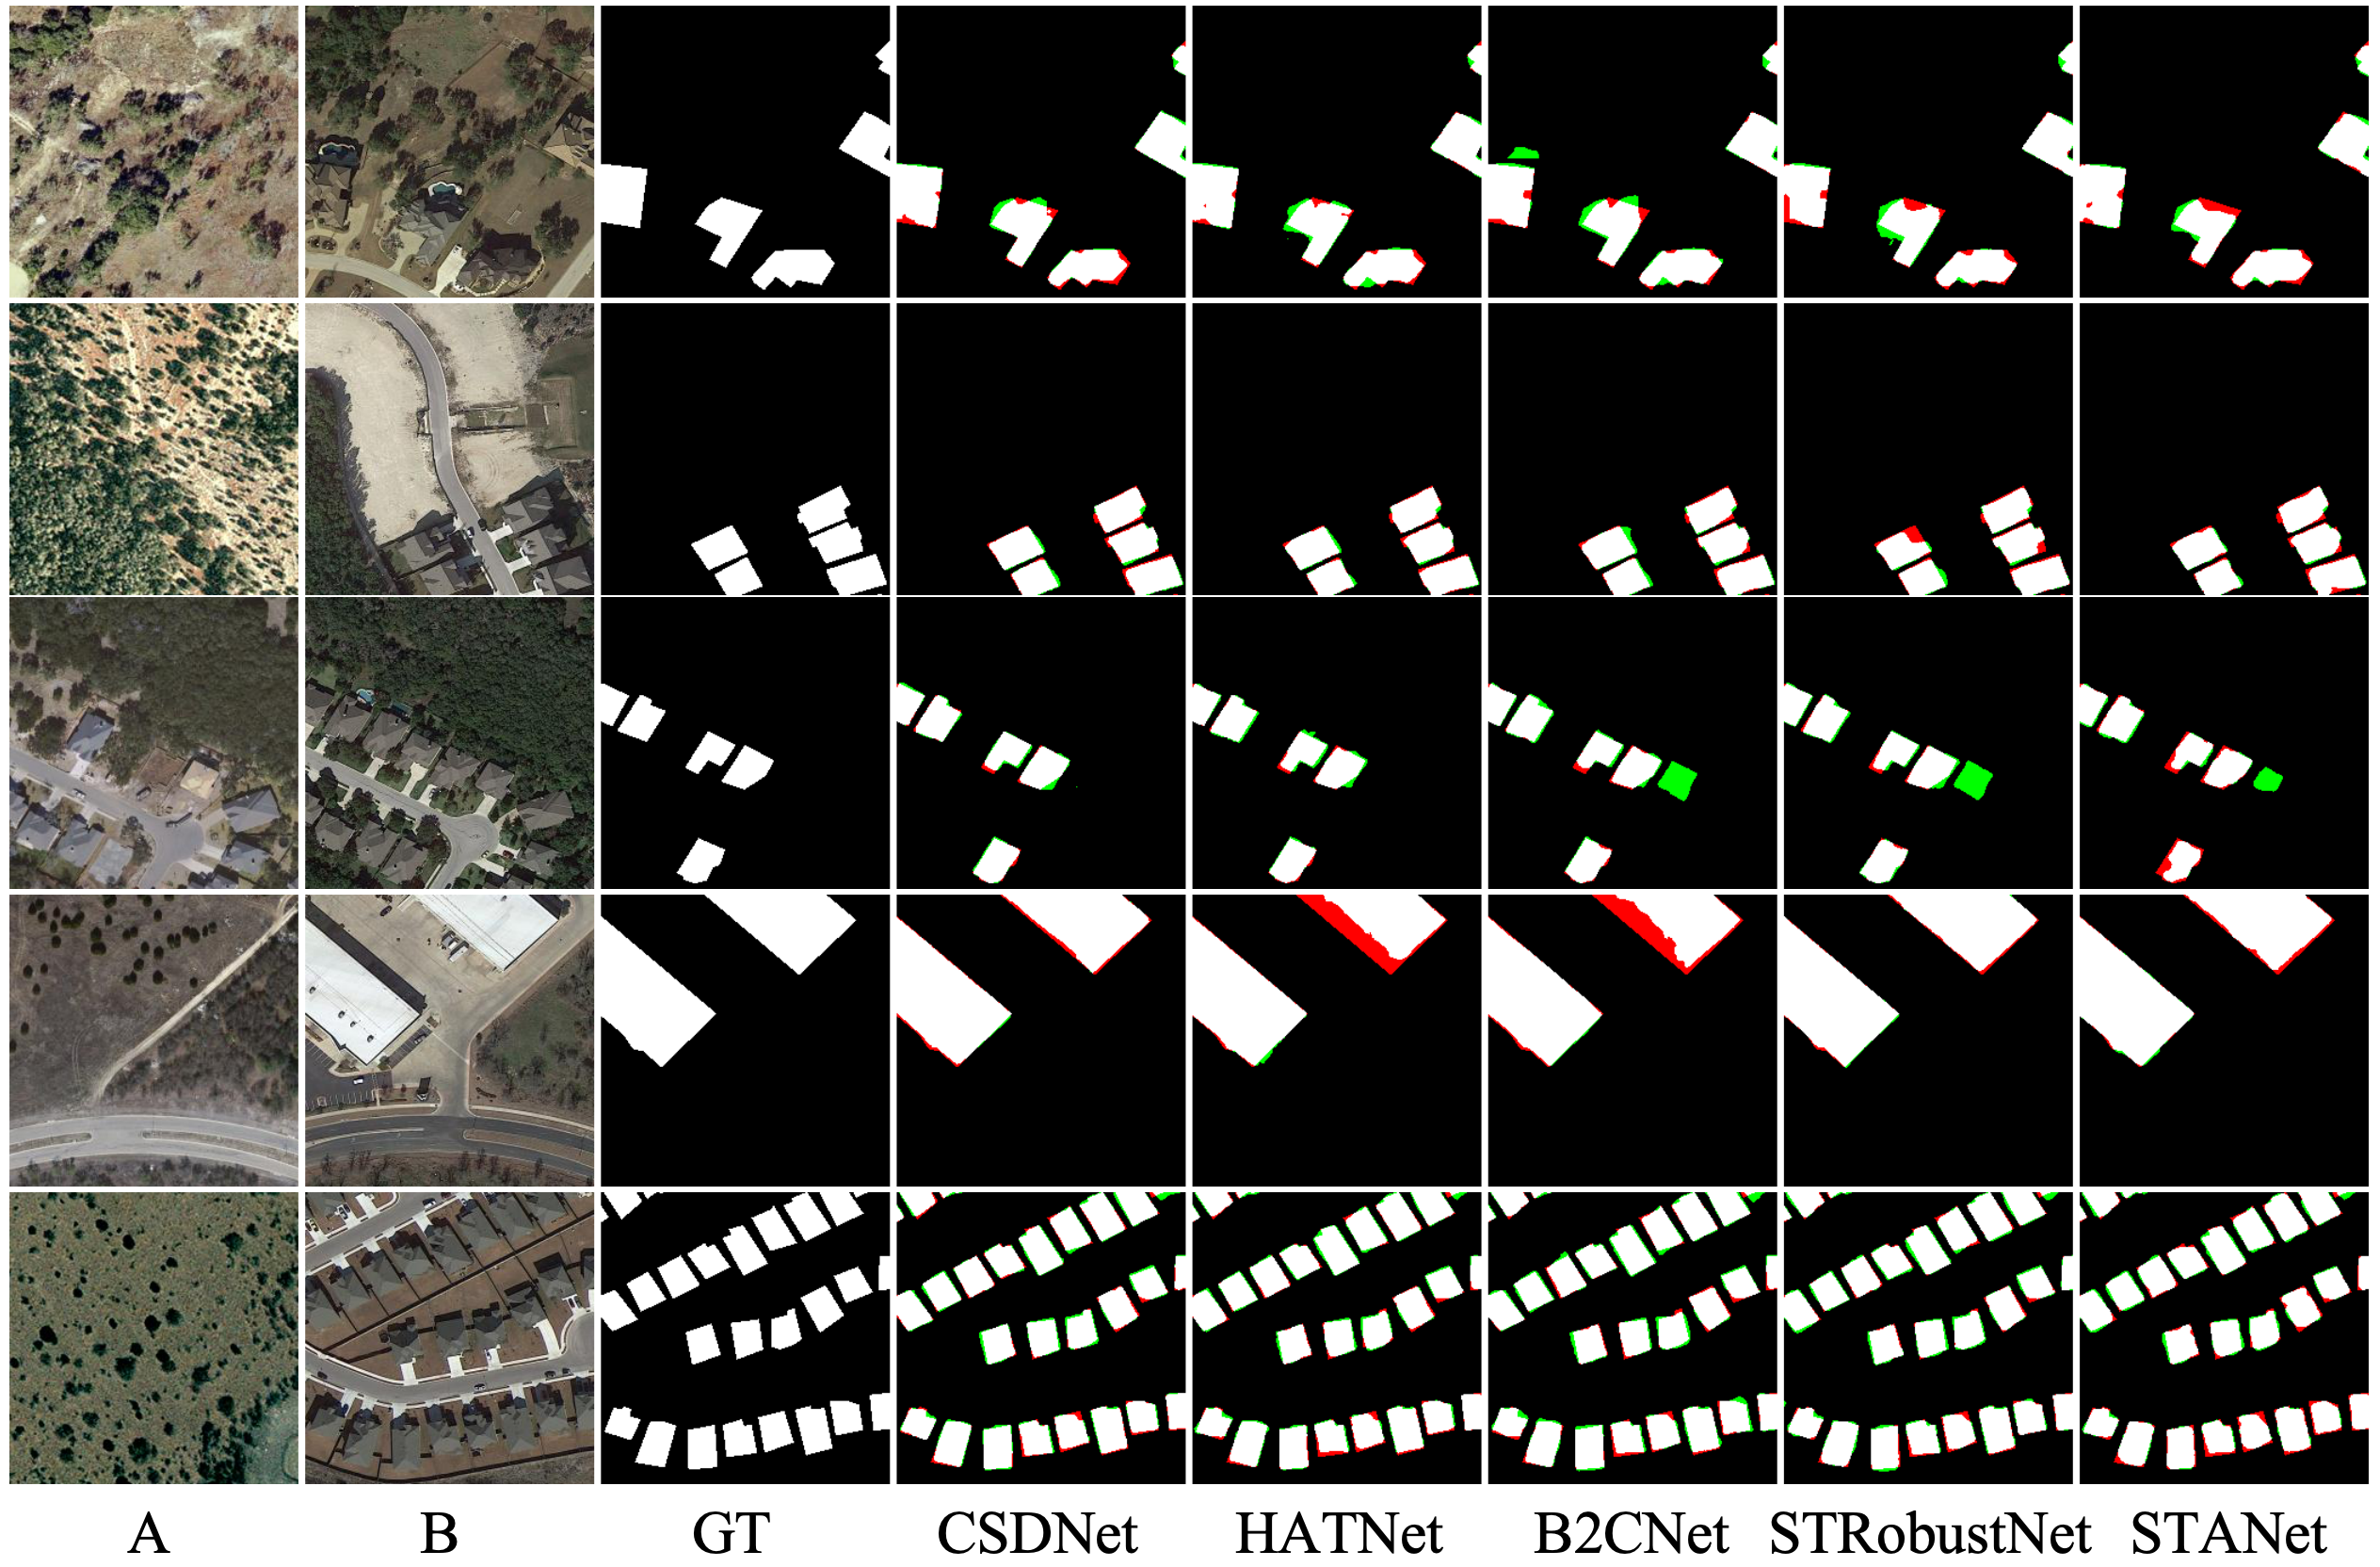
\includegraphics[width=\linewidth]{paper_figures/基于双时相遥感影像风格解缠和内容细化增强遥感变化检测方法/csdnet_levir.png}
    \caption{CSDNet 模型与经典模型在 LEVIR-CD 测试集上的可视化对比结果}
	\label{fig:csdnet_levir}
\end{figure}

\begin{table}[!htbp]
\centering
\caption{CSDNet 模型与经典模型在 LEVIR-CD 数据集上的定量对比结果}
\label{tab:csdnet_levir}
\resizebox{\linewidth}{!}{%
% 这里是关键修改:将所有的 S[...] 列类型改为了 c (居中)
\begin{tabular}{l c c c c c} 
\toprule
Method & {OA} & {IoU} & {F1} & {Recall} & {Precision} \\
\midrule
CDNet~\cite{Alcantarilla2016StreetviewCD} & 98.35 & 72.21 & 83.87 & 84.14 & 83.61 \\
BIT~\cite{chen_remote_2022} & 98.95 & 80.86 & 89.48 & 87.53 & 90.65 \\
STANet~\cite{chen_spatial-temporal_2020} & 99.02 & 81.85 & 90.02 & 87.13 & 93.10 \\
MSCANet~\cite{m_liu_cnn-transformer_2022} & 99.03 & 81.91 & 90.06 & 86.38 & 94.06 \\
MFATNet~\cite{Mao2022MFATNetMF} & 99.03 & 82.42 & 90.36 & 88.93 & 91.85 \\
ChangeFormer~\cite{bandara2022transformer} & 99.04 & 82.66 & 90.50 & 90.18 & 90.83 \\
P2V~\cite{lin_transition_2023} & 99.04 & 83.00 & 90.71 & 91.78 & 89.67 \\
AMTNet~\cite{Liu2023AnAM} & {--} & 83.08 & 90.76 & 89.71 & 91.82 \\
MSNet~\cite{Liu2025NetworkAD} & 99.14 & 83.60 & 91.41 & 89.99 & 92.87 \\
STRobustNet~\cite{Zhang2025STRobustNetEC} & 99.10 & 83.66 & 91.11 & 90.67 & 91.54 \\
B2CNet~\cite{Zhang2024B2CNetAP} & 99.10 & 83.72 & 91.14 & 91.01 & 91.27 \\
ChangeCLIP(ViT-B/16)~\cite{dong2024changeclip} & 99.14 & 83.99 & 91.30 & 89.04 & 93.68 \\
HATNet~\cite{Xu2024HybridAT} & 99.13 & 84.12 & 91.38 & 90.15 & 92.64 \\
DMATNet~\cite{Song2022RemoteSI} & 98.25 & 84.13 & 90.75 & 89.98 & 91.56 \\
STransUNet~\cite{Yuan2022STransUNetAS} & 99.13 & 84.19 & 91.41 & 90.55 & 92.30 \\
\textbf{CSDNet} & \textbf{99.16} & \textbf{84.47} & \textbf{91.58} & \textbf{90.00} & \textbf{93.23} \\
\bottomrule
\end{tabular}%
}
\end{table}


\begin{table}[!htbp]
\centering
\caption{CSDNet 模型的消融实验结果 (IoU \%)}
\label{tab:csdnet_ablation}
\resizebox{\linewidth}{!}{%
\begin{tabular}{ccccccc}
\toprule
\textbf{CSDM} & \textbf{CCRM} & \textbf{SYSU-CD} & \textbf{LEVIR-CD} & \textbf{WHUCD} & \textbf{MSRSCD} & \textbf{S2Looking} \\
\midrule
$\times$ & $\times$ & 70.30 & 83.62 & 89.78 & 59.95 & 49.88 \\
$\checkmark$ & $\times$ & 70.59 & 83.94 & 90.22 & 61.46 & 50.31 \\
$\times$ & $\checkmark$ & 70.64 & 83.85 & 90.38 & 60.88 & 50.22 \\
$\checkmark$ & $\checkmark$ & \textbf{71.16} & \textbf{84.47} & \textbf{90.88} & \textbf{62.01} & \textbf{50.72} \\
\bottomrule
\end{tabular}%
}
\end{table}

\begin{table}[!htbp]
\centering
\scriptsize
\setlength{\tabcolsep}{3pt} % 调整列间距
\caption{CSDNet 模型在五个数据集上训练前后的 UMAP 嵌入域差异度量。负增量表示训练后度量下降(通常表示域间隙减小)。}
\label{tab:domain_metrics_transposed_improved_delta}
\begin{tabular}{l l c c c c c}
\toprule
Metric & Stage & {WHUCD} & {MSRSCD} & {S2Looking} & {LEVIR-CD} & {SYSU-CD} \\
\midrule
\multirow{3}{*}{Centroid dist} 
  & Before training & 9.5444 & 1.0438 & 8.1495 & 7.2442  & 13.0549 \\
  & After training  & 7.8133 & 1.2386 & 7.5414 & 2.8456  & 11.2671 \\
  & $\Delta$ & \textcolor{red}{\textbf{-1.7311}} & \textcolor{blue}{\textbf{+0.1948}} & \textcolor{red}{\textbf{-0.6081}} & \textcolor{red}{\textbf{-4.3986}} & \textcolor{red}{\textbf{-1.7878}} \\
\midrule
\multirow{3}{*}{MMD} 
  & Before training & 0.1655 & 0.0526 & 0.1053 & 0.2022 & 0.3706 \\
  & After training  & 0.1213 & 0.0560 & 0.0953 & 0.1229 & 0.1448 \\
  & $\Delta$ & \textcolor{red}{\textbf{-0.0442}} & \textcolor{blue}{\textbf{+0.0034}} & \textcolor{red}{\textbf{-0.0100}} & \textcolor{red}{\textbf{-0.0793}} & \textcolor{red}{\textbf{-0.2258}} \\
\midrule
\multirow{3}{*}{CORAL} 
  & Before training & 821.4465  & 384.3917  & 1941.6185 & 3277.2930 & 820.3972 \\
  & After training  & 1502.2324 & 326.6985  & 1338.1335 & 1628.3154 & 451.8247 \\
  & $\Delta$ & \textcolor{blue}{\textbf{+680.7859}} & \textcolor{red}{\textbf{-57.6932}} & \textcolor{red}{\textbf{-603.4850}} & \textcolor{red}{\textbf{-1648.9776}} & \textcolor{red}{\textbf{-368.5725}} \\
\bottomrule
\end{tabular}
\end{table}

\section{讨论}

\subsection{内容-风格解耦与变化敏感性}
内容-风格解耦模块 (CSDM) 在减轻双时相图像的风格干扰和增强变化敏感性方面展现了实证有效性。如表~\ref{tab:domain_metrics_transposed_improved_delta} 所示,计算了训练前后特征在 UMAP 嵌入空间上的三种域差异度量——质心距离 (centroid distance)、最大均值差异 (maximum mean discrepancy, MMD) 和 CORAL。这些指标量化了双时相图像特征分布的对齐程度,数值越低表明对齐效果越好,风格噪声越少。

引入 CSDM 后,UMAP 嵌入空间中的质心距离和 MMD 在多数数据集上均显著下降(例如,在 SYSU-CD 上,质心距离从 13.0549 降至 11.2671,MMD 从 0.3706 降至 0.1448),这表明双时相特征分布在几何中心和再生核空间层面的差异被压缩,即风格/域偏移被有效抑制。CORAL 指标在多个数据集(如 MSRSCD、S2Looking 和 LEVIR-CD)上也呈现下降趋势,反映了解耦后协方差结构的一致性得到了更好的重构;而在 WHUCD 上 CORAL 的上升可能表明,CSDM 在移除显式风格噪声的同时,对原始协方差进行了结构性重塑,以保留或适应有用的细粒度统计信息。总体而言,这些量化变化支持了 CSDM 的设计初衷:通过实例归一化和通道门控,它选择性地移除了无关的风格因素(如光照、季节和传感器噪声),同时保留了边缘、纹理等有益的风格线索,从而提高了模型对真实变化的判别能力。该模块不仅在特征表示上实现了更好的对齐,也带来了更鲁棒的变化检测性能。

\subsection{上下文内容精炼与边界清晰度}
除了内容-风格解耦模块 (CSDM) 在特征编码阶段对风格噪声的有效抑制,还在解码阶段引入了上下文内容精炼模块 (CCRM),以实现变化区域的精细化勾勒。CCRM 的核心在于其联合通道和空间门控机制,该机制在恢复特征分辨率的同时,对残余的风格特征进行二次筛选和重组。这一机制使得模型能够更专注于具有显著变化信号的区域,同时抑制可能导致假阳性的局部纹理或噪声,从而生成更精确的变化图。

通过 CSDM 和 CCRM 的协同工作,CSDNet形成了一个完整的“先粗滤后精炼”的工作流。CSDM 在前期处理全局的风格差异,为解码器提供了更纯净、更稳定的内容特征。在此基础上,CCRM 在特征重构过程中进行局部和上下文层面的优化,确保最终输出的变化边界清晰、完整,并显著减少了假阳性与假阴性。如可视化结果所示,与其它方法相比,CSDNet 在复杂场景中能更准确地勾勒出变化物体的轮廓,验证了这种编码器-解码器协同作用在提升变化检测精度和鲁棒性方面的优越性。


\section{本章小结}

本章提出了一种基于内容-风格解耦和通道-空间门控的双时相变化检测网络 CSDNet。在编码阶段,网络利用内容-风格解耦模块 (CSDM) 对多尺度特征进行实例归一化和风格残差提取,并通过通道门控自适应地保留有助于变化检测的风格线索。在解码阶段,上下文内容精炼模块 (CCRM) 对风格残差进行通道和空间双重门控精炼,然后与内容特征进行重组,显著提升了变化边界的清晰度和检测精度。实验结果表明,在 LEVIR-CD、SYSU-CD、WHUCD、S2Looking 和 MSRSCD 数据集上,CSDNet 在 F1、IoU 和精度指标上均优于多种先进的 SOTA (State-of-the-art) 方法,验证了所提模块在复杂地物背景下的高度鲁棒性和准确性。
